% latexmk -pvc -pdf
\documentclass[a4paper]{article}
\usepackage[margin=0.65in]{geometry}
\usepackage{multicol}
\usepackage{amsthm,amsfonts,amssymb}
\usepackage[english]{babel}
\usepackage{blindtext}
\usepackage{sidecap}
\usepackage{caption}
\usepackage{subfig}
\usepackage{graphicx}
\newenvironment{Figure}
    {\par\medskip\noindent\minipage{\linewidth}}
    {\endminipage\par\medskip}
\newenvironment{itemizeReduced}{
\begin{list}{\labelitemi}{\leftmargin=1em}
\setlength{\itemsep}{1pt}
\setlength{\parskip}{0pt}
\setlength{\parsep}{0pt}}{\end{list}
}

\title{
    
}
\author{Ana C. Fabela Hinojosa \\
\small{School of Physics and Astronomy, Monash University}}
\date{Last edit: \today}

\begin{document}
\maketitle

\begin{abstract}
We investigate how the range of alpha particles changes as the alpha particles interact with a surrounding medium. The experiment aims to describe the observed energy spectrum for alpha particles emitted from a radioactive \textsuperscript{241}Am source. By increasing air pressure in a sealed vacuum chamber we are able to determine the straggling parameter of the travelling particles to be $\alpha = 0.15 \pm 0.01 cm$. In this investigation we also calculate the thickness ($\Delta x = 2.45 \pm 0.08\mu$) of the gold overcoat layer that is part of the radioactive source construction, we compare our result to the manufacturer value $3\mu$m. and Finally from our data we are able to determine the range pressure is $p_0 = 39.72 \pm 0.18$kPa.

\end{abstract}

\section{Introduction}

\begin{multicols}{2}

The least penetrating type of ionizing radiation consists of two protons and two neutrons (nucleons) bound together in alpha particles.\cite{SPA, alpha}

When an atom's nucleus emits an alpha particle, the atom's mass number decreases by four due to the loss of the four nucleons that make the alpha particle\cite{alpha}. 
In this type of decay event, the created alpha particle and daughter nucleus must balance out the strong force (given the nuclear scale) with newly aquired coulomb repulsion (both the daughter nucleus and alpha particle have net positive electric charges). It is natural that the coulomb repulsion overtakes the strong force leading to the alpha particle being eventually ejected form the nucleus.

As the alpha particle moves through matter and because of it's net positive charge, the ejected alpha particle will interact by means of the coulomb force with the surrounding medium. The travelling particle thus loses kinetic energy in many steps, until it's energy approaches zero.  which will lead to a kinetic energy loss.\cite{SPA}. The travelled distance is called the range of the particle\cite{straggling}.

\subsection{Detection of alpha particles}
When an incident charged particle enters the detector, electron-hole pairs are created as the particle is descelerated. The charges are drawn to the appropriate surface contact, crating a charge pulse that is proportional to the energy of the charged particle.\cite{SPA}
In this experiment we use a pulse amplifier to convert charge-to-voltage, providing us an output voltage that is proportional to the charge produced by the input photo diode\cite{SPA}.
We detect the voltage pulses with the multichannel analyser, and record the pulses heights in a series of internal bins producing a histogram.\cite{SPA}

\section{Background Theory}
Alpha particles do not have enough kinetic energy to escape the potential well from the strong force inside the nucleus. Nevertheless, due to quantum tunnelling and the coulomb repulsion effect, the created alpha particles spend some time in a region so far from the nucleus that the potential from the repulsive electromagnetic force has fully compensated for the attraction of the nuclear force.
Causing the ejection of the particle from the nuclear region\cite{alpha}.  
 
\subsection{The decay path of \textsuperscript{241}Am}
The most probable alpha decay event observed in this experiment occurs with $85\%$ probability. The mean life of \textsuperscript{241}Am is 458 years\cite{SPA}.

An \textsuperscript{241}Am nucleus decays to a \textsuperscript{237}Ne, a \textsuperscript{4}He nuclei and a gamma ray with $E = 59.6$ keV\cite{americium}.
\subsection{The range of \textsuperscript{241}Am}
In 1933 Hans Bethe developed the Bethe formula which describes the mean energy loss per distance travelled by charged particles\cite{Bethe}

\begin{equation} \frac{-\mathrm{d} E}{\mathrm{d} x} = B \rho E_0^{- 0.73}
\end{equation}

where $B = 2.58$ MeV (cm kg m\textsuperscript{-3})\textsuperscript{-1}, $E_0$ is the initial kinetic energy of the alpha particle, the density of air at $20^{\circ}$C and $101.325 $kPa: $\rho = 1.204$ kgm\textsuperscript{-3} and finally x is the distance travelled by the particle in cm\cite{SPA}.

We can integrate equation (1) with respect to distance to obtain the range of the alpha particles as a function of initial energy
\begin{equation} R = \frac{E_0^{1.73}}{1.73 B \rho}
\end{equation}
This allows us to calculate a theoretical expression for the range at one atmosphere\cite{SPA}
\begin{equation} R_{atm} = 0.186 E_0^{1.73}
\end{equation}

Since energy loss is proportional to the number of gas molecules encountered\cite{SPA}, we use 
\begin{equation} R = R_{atm} \frac{P_{atm}}{P},
\end{equation}
where $P$ is the pressure and $P_{atm}$ is the atmospheric pressure, assuming that air behaves as an ideal gas this implies that the density of air molecules will vary linearly with the pressure P\cite{SPA} as per the following expression
\begin{equation} \rho = \frac{P}{R_d T},
\end{equation}
where T is the absolute temperature of the gas and $R_d = 287.05$J(kg K)\textsuperscript{-1} is the specific gas constant.
Using this relation the range R becomes:
\begin{equation} R = 64.31 \frac{T}{p} E_0^{1.73},
\end{equation}
where the initial mass-energy $(E_0)$ is measured in MeV\cite{SPA}. 

\subsection{Range straggling}
All alpha particles have the same initial mass-energy. It's likely that the reader might assume that if the emitted alpha particles interact with a homogeneous medium their ranges should be identical.

Nevertheless, experiments show that random variations in the effective path lengths occur due to the molecular nature of air. Which leads us to consider the statistical nature of such interactions. The number of collisions required to bring an alpha particle to rest within the medium will vary slightly, depending on the number of collisions the particle suffers.
Hence, there will be a small variation in the particle's range. This is known as straggling\cite{straggling}.

It is also important to mention why the approach of varying the pressure in the chamber is used instead of modifying the distance between the source and the detector.
Both approaches are theoretically identical but for practical purposes a fixed chamber size is used. Another geometric consideration is that modifying the distance to the detector changes the solid angle of the ejected alpha particles; changing the number detected particles independently of other loss mechanisms\cite{feedback}.

To determine the full straggling parameter $(\alpha)$, we must consider an additional dispersion in the energy spectrum. Occuring due to the construction of the radioactive source used in this experiment. 
The source has a layer of gold that covers the surface where the radioactive source rests\cite{SPA}. 

Thus we write our expression for the straggling parameter as the sum\cite{SPA}
\begin{equation} \alpha^2 = \alpha_{air}^2 + \alpha_{source}^2,
\end{equation}

where the straggling parameter of alpha particles in air $(\alpha_{air})$ is characterised by\cite{SPA} 
\begin{equation} \alpha_{air} = 0.6006 FWHM,
\end{equation}
here FWHM is the "full width half maximum" of the observed distribution that is the energy spectrum. 



We examine the number of alpha particles as the pressure chamber is varied using
\begin{equation} n(p) = \frac{n_0}{2} \left (1- erf \left (\frac{p - p_0}{\alpha}\right )\right ),
\end{equation}
where p is the varying air pressure in the chamber, $n_0$  is a large number of particles with initial velocity $(v_0)$ (this parameter will be useful for normalisation), $p_0$ is the pressure preventing alpha particles from reaching the spatially fixed detector ($x_0$ cm away from the radioactive source) and $\alpha$ is the full straggling parameter we defined earlier\cite{SPA}.

\subsection{Bragg--Kleeman rule}
As we described in section 2.3 in order to determine the correct straggling parameter in our experiment we must correct for the construction of the radioactive source. The effective stopping power of materials other than air is approximately inversely proportional to $\rho$ the density and $\sqrt{A}$ where $A$ is the atomic mass of the substance through which the alpha particle travels.

The Bragg--Kleeman rule is used to predict the energy loss for alpha particles passing through a material by comparing it to a reference material. It is generally known to be accurate to within $\pm 15\%$\cite{SPA}, in terms of comparing ranges we write the rule as
\begin{equation} \frac{R_1}{R_0} = \frac{\rho_0}{\rho_1}\sqrt{\frac{A_1}{A_0}},
\end{equation}

where $R_0$is the range of the alpha particles in the reference material and $R_1$ is the range of the alpha particles in the some other arbitrary material.
In this experiment the reference material used is air.

The values used for $\sqrt{A_0} = \sqrt{A_{air}} = 3.82$ and $\rho_0 = 1.204$ kgm\textsuperscript{-3}\cite{SPA}. We calculated the $R_0 = R_{atm} = 2.47 \pm 0.08$cm using equation (3).

We use equation (9) to find the range of alpha particles travelling through gold given the layered construction of our radioactive source. We require an expression to predict the energy loss from alpha particles travelling through the gold layers of the construction (by a distance $\Delta x$). 
From integrating equation (1) we obtain
\begin{equation} E = \left(E_0^{1.73} -0.0156 \rho \frac{\Delta x}{T} \right)^{0.578},
\end{equation}
here we can use equation (9) again and replace $\rho =  \rho_1\sqrt{\frac{A_{air}}{A_1}}$
\begin{equation} \therefore E = \left(E_0^{1.73} - 0.0156 \rho_1\sqrt{\frac{A_{air}}{A_1}} \frac{\Delta x}{T} \right)^{0.578},
\end{equation}
where $\rho_1 = \rho_{gold} = 19.30 (g / cm^3), A_1 = A_{Au} = 196.97$ are the density and atomic mass of gold\cite{gold}.

From these relationships we find that the energy of alpha particles after passing through a thickness $\Delta x$ of gold is found by\cite{SPA}
\begin{equation} E = \left(E_0^{1.73} -4.464 \rho_1\sqrt{\frac{A_{air}}{A_{Au}}} \Delta x \right)^{0.578}.
\end{equation}



\section{Method}
The experimental set up allows for the acquisition of data pulses that have pulse height greater than 10 bins for 300s in 1024 bins. 
This bin number has been chosen to optimise for an adequate signal to noise ratio as well as resolution of the spectrum.
The MCA device will only record a new pulse after the input voltage drops below the threshold level\cite{SPA}.
Below we outline the procedure followed in order to configure our experimental apparatus for optimal operation. 

\subsection{Alpha particle detection}
To configure our detector, we by turn "on" the power switch of the "NIM" bin and turning "on" the MCA and DSO amplifier units.
\subsection{Adjusting chamber pressure}
The chamber pressure is controlled by admitting air into the chamber using the "air admit" valve. If partial evacuation of the chamber is required, repeat the steps described next.
We first close the air admittance valve and proceed to turn "on" the vacuum gauge. We activate the pump and open the "Vacuum pump line". The aparatus will start removing air from the chamber, once the pressure is below $0.05$kPa we close the "Vacuum pump line" and finally we deactivate the pump. 
We proceed by ensuring that the amplifier output is connected to DSO the particle pulses are detected to be approximately $> 2V$. Finally, we make sure the amplifier output is connected to MCA unit

\subsection{MCA software set-up}
In order to operate the detector we must launch "ADMCA" software. Once we start the software in the computer an initialisation menu will require us to accept default device (MCA8000A) attached to the computer and the experimental apparatus. we click "connect" and proceed by adjusting the data acquisition settings.
In the MCA menu we click 'Acquisition set up' and we ensure preset mode is set to 'seconds'. After this we proceed to ensure that the timer is set to 'live time' with preset time t = 100s.
The 'threshold' is set to 42 (Please Note that the threshold value might have to be readjusted) and the 'ADC channels' to '1024'.

After this configuration is set we click 'ok' to preserve this settings.
The final steps are to clear any data stored in the MCS memory by clicking in the MCA menu "Delete data and Reset time" and finally we 
click in the MCA menu the "Start acquisition" option to begin with our data acquisition.

To visualise our data, we defined a region of interest (ROI) for the software. Clicking "edit ROI" on the toolbar and dragging a cursor over the region containing the visible peak. We exit this tool by clicking "edit ROI" once again. The spectra is saved in an ASCII file format which we analysed using python.
As the pressure increases the alpha particle spectrum moves towards the lower energy region and the spectrum skews. It is necessary that we estimate the peak position for each spectrum.

In order to find a representative value for the peak of each spectra we processed our data using a gaussian smoothing technique. We simply convolved the raw data with a gaussian that has $\sigma = 4$ From this it was straight forward to find an estimate for the mean of each distribution.
We calculate an uncertainty estimate for this process by observing the data and estimating the possible uncertainty in the computed mean form the smoothed data. We also calculated a rough uncertainty in the  mean count by observing the size of our noise and dividing this by the square root of the number of bins present in the FW of the gaussian used for the convolution.
The uncertainty in the bin position of the mean (peak position $\pm$ 8)is the same as the vertical uncertainty in figure 3 in the analysis.
We also use the smoothed data to find the FWHM of each of the smoothed spectra. The uncertainty in the FWHM is estimated visually.

\subsection{Detector's Zero energy}
The output for the detector's zero signal does not necessarily correspond to zero volts. In addition to this, the first bin of the MCA spectrum will not necessarily correspond to the zero input signal\cite{SPA}.

To find the baseline signal of the detector it is useful to fill  the  chamber  with  air  completely as this will  stop  all  alpha  particle detection events\cite{SPA}.
The  MCA  unit’s detection range is set between 0 and 5 volts, therefore we assume that the first and last bins in the MCA range correspond exactly to a 0 and 5 volt input respectively and we proceed to calibrate the visible x axis. 

Converting the measured voltage into an anticipated MCA bin value requires us to multiply the x-axis by the estimated size of each bin.
We therefore correct your data by considering the background count offset using the calibrated x-axis, and the threshold observed.

Another important factor for obtaining an adequate spectrum is to make sure the threshold used is set to cut out the majority of the background noise peak. This presents a problem since the obtained spectrum of the particles fails to be complete at low energies given the cutting out of the noise peak. We fix this issue by extrapolating the spectrum.To do this, we choose to take an average of the first 50 values above the threshold for each unprocessed (ie. not gaussian smoothed) data set and assigning this average value to all the "zero valued" bins below the threshold.
By doing this we obtain a representative curve that accounts for the shape and noise of our data. The respective extrapolations are then plotted in the "gaussian smoothed" spectrum plots for each data set.

\subsection{Data acquisition parameters}
\begin{itemizeReduced}
    \item Laboratory temperature $T = 294.15 \pm 0.5 K$
    \item MCA threshold $ = 42$
    \item Acquisition time $t = 100s$
    \item Background threshold: $4$
\end{itemizeReduced}
\end{multicols}

\clearpage
\section{Results}
\begin{figure}[!htbp]
\subfloat[]{\scalebox{0.37}{
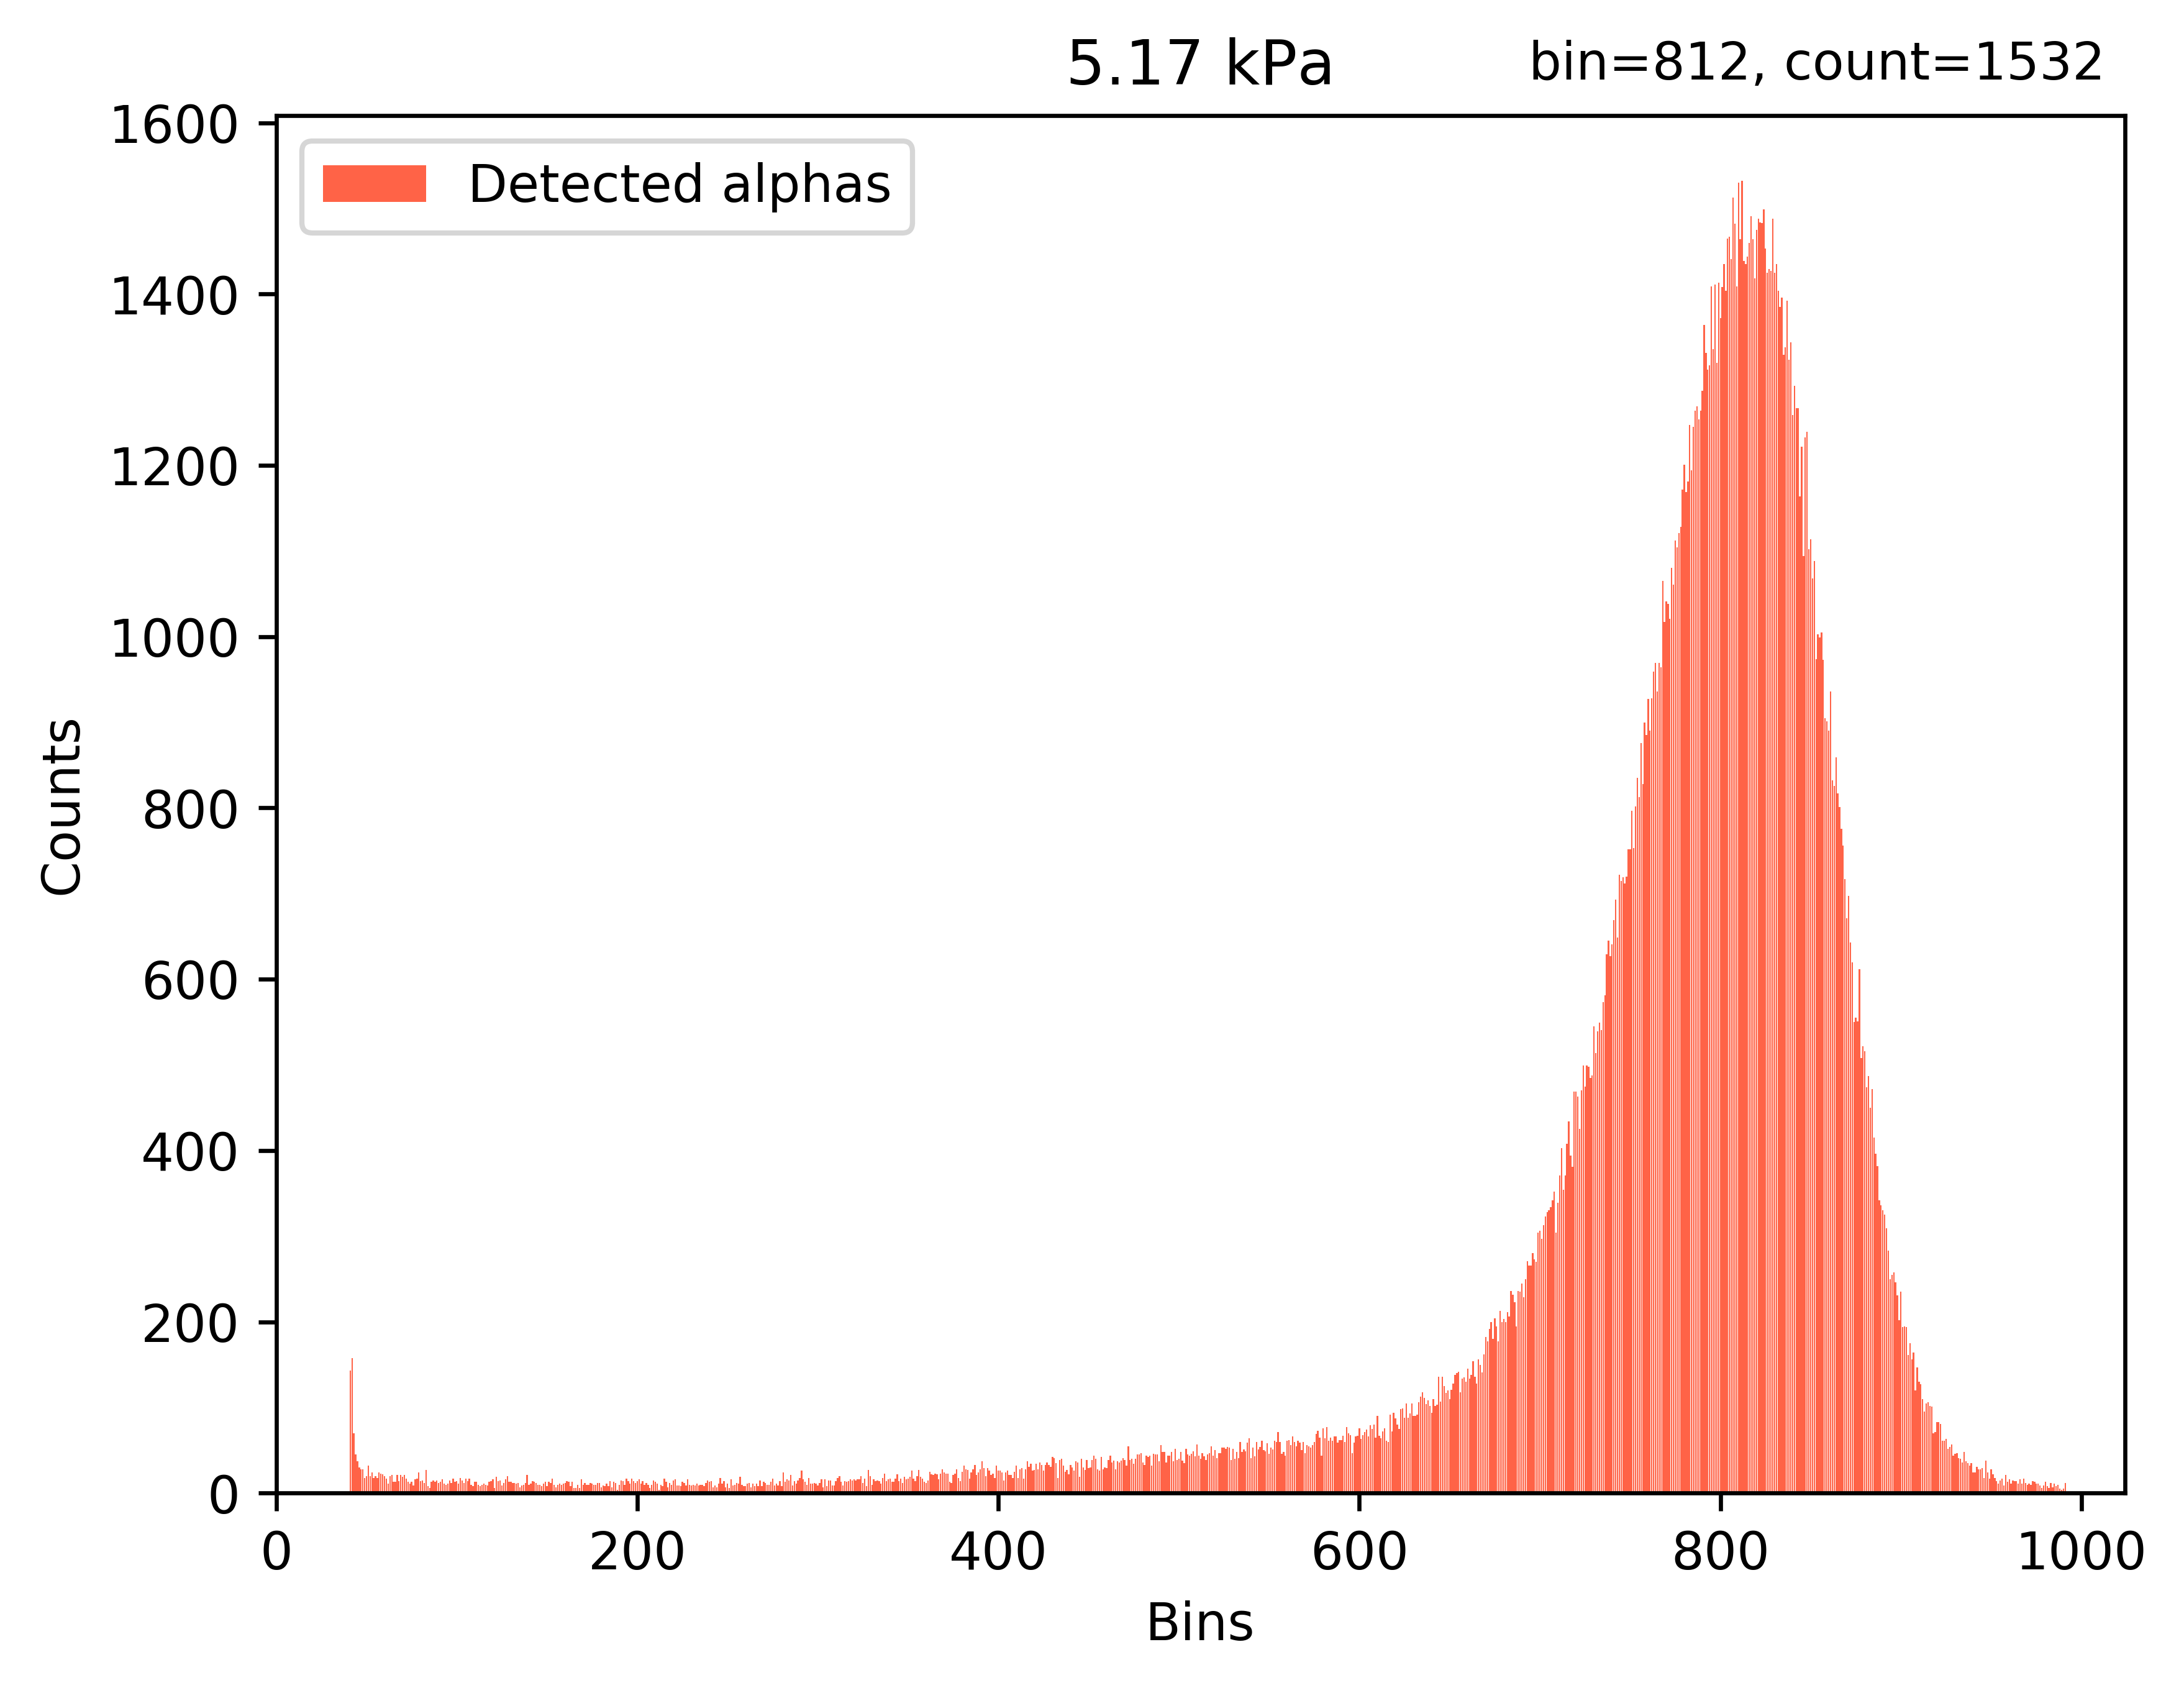
\includegraphics{raw_p=5.17kPa.png}    
}}
\subfloat[]{\scalebox{0.37}{
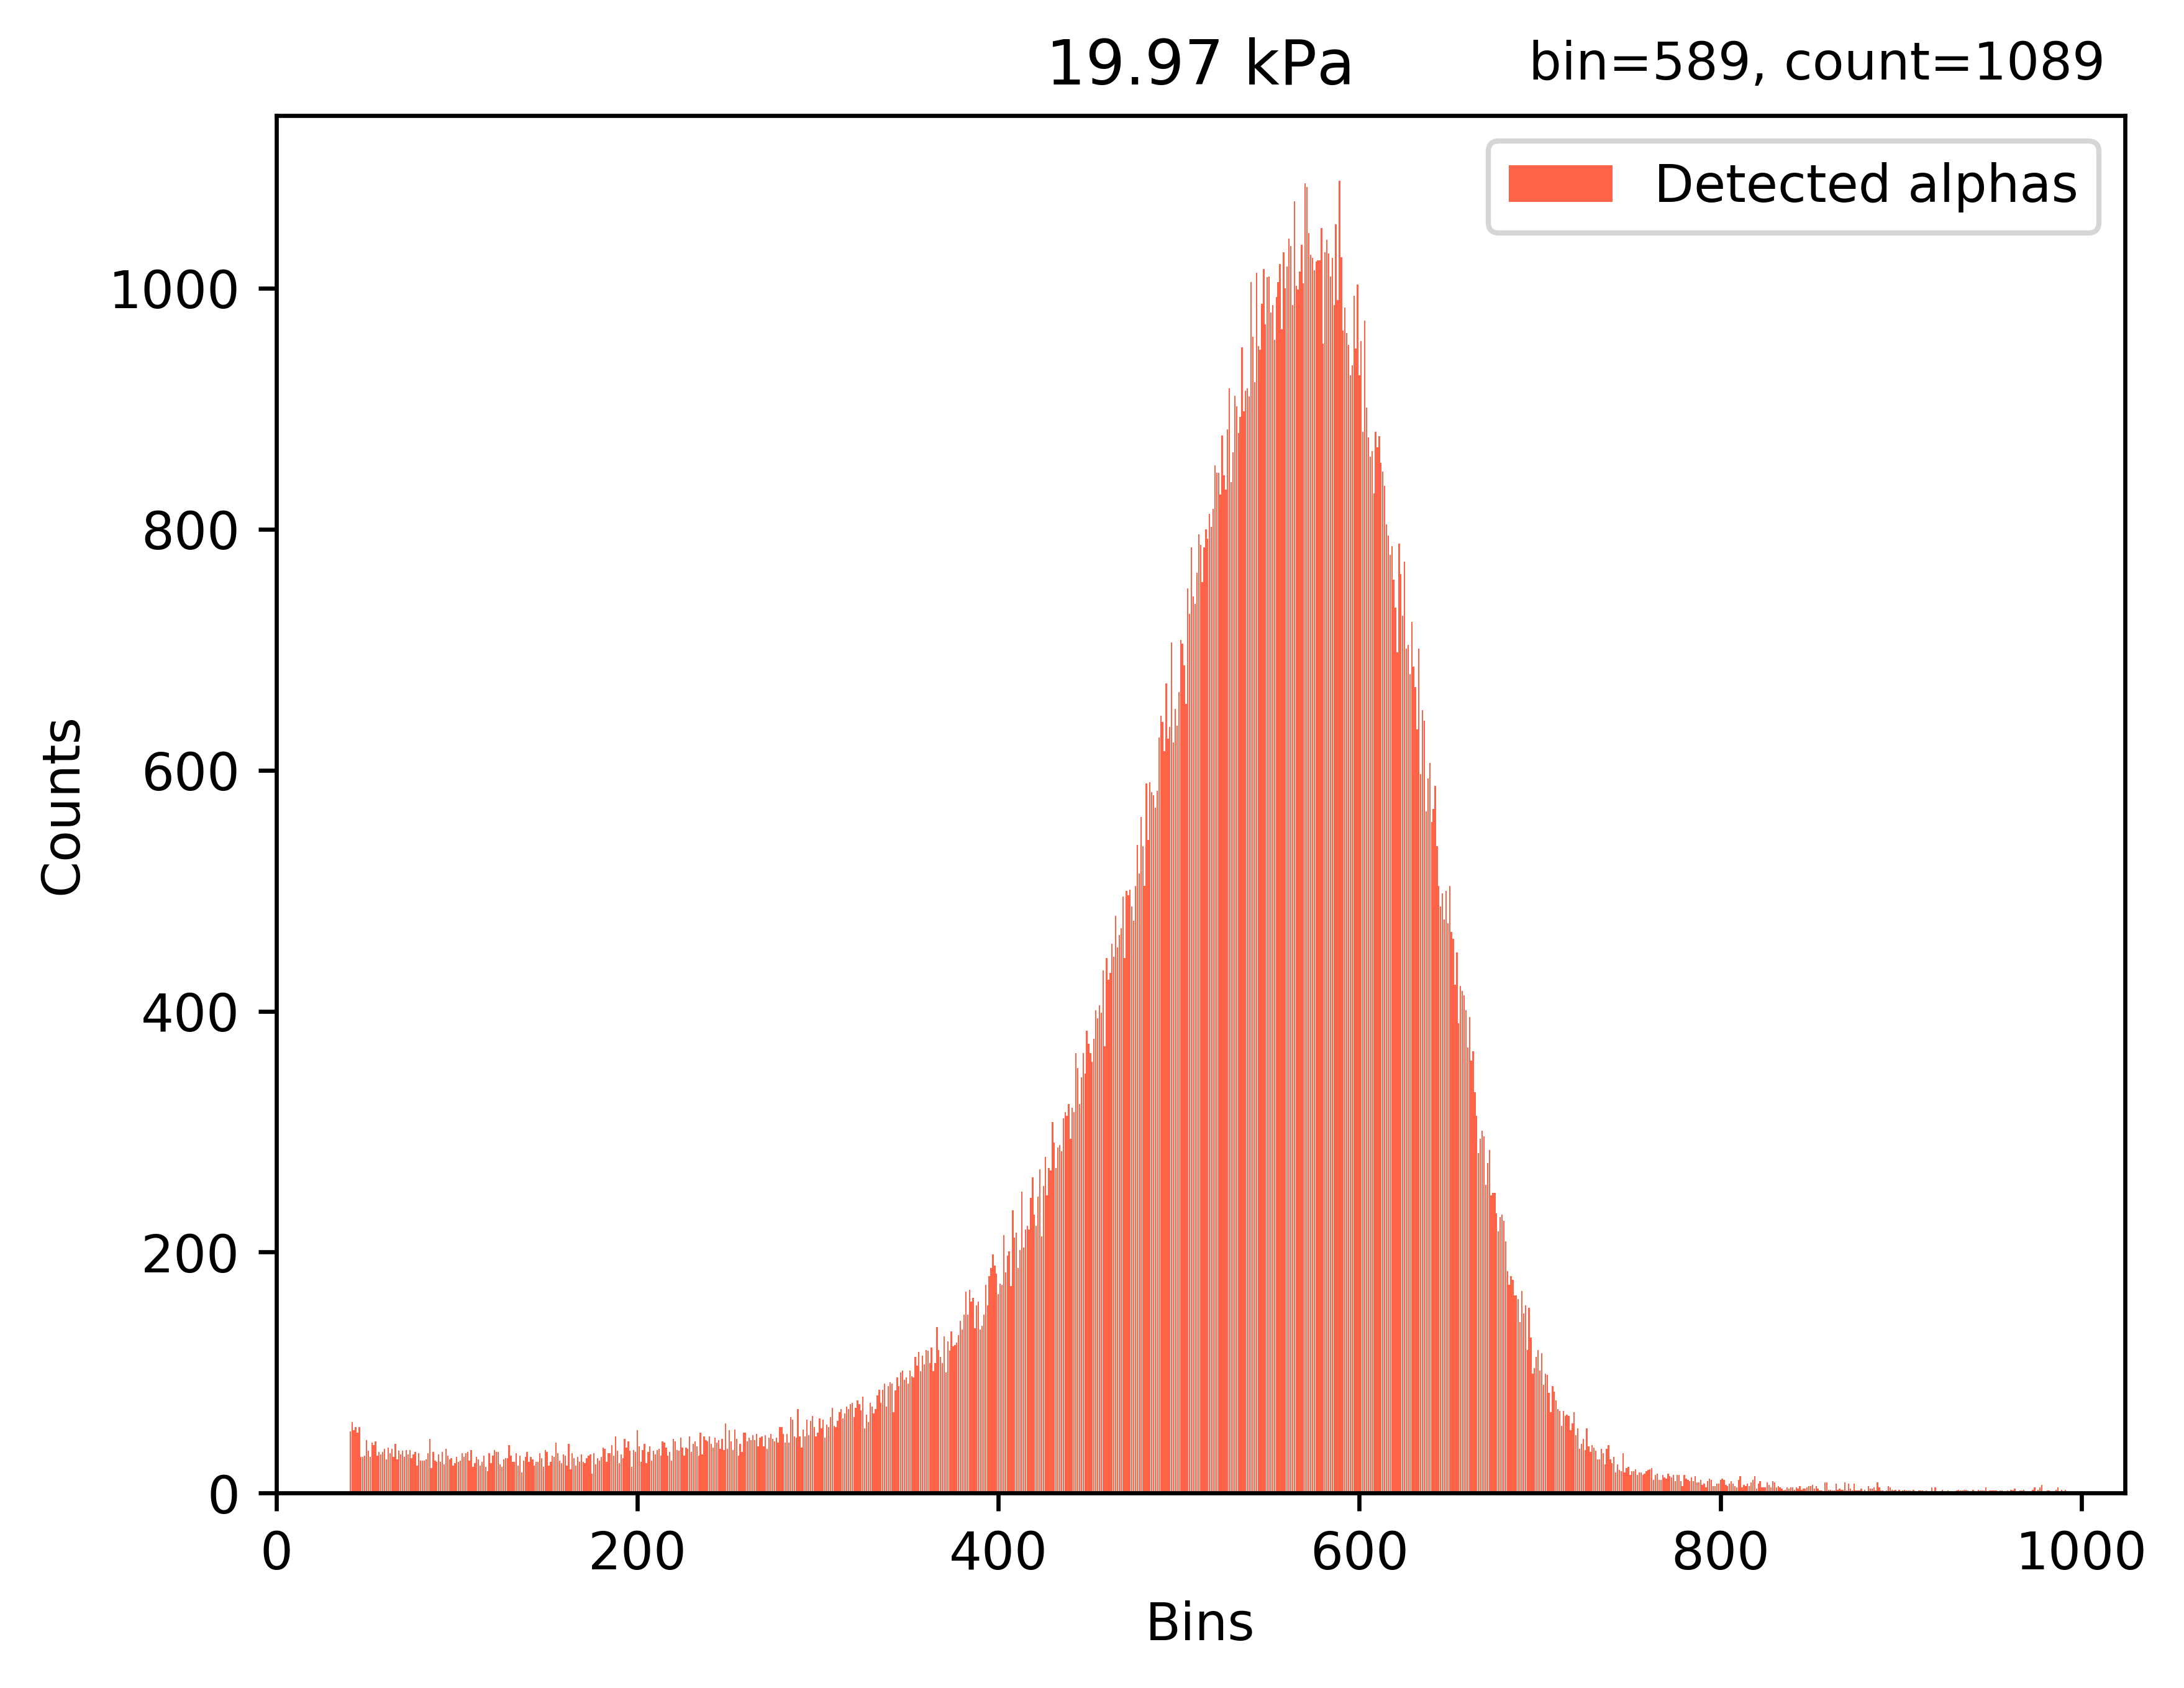
\includegraphics{raw_p=19.97kPa.png}   
}}
\subfloat[]{\scalebox{0.37}{
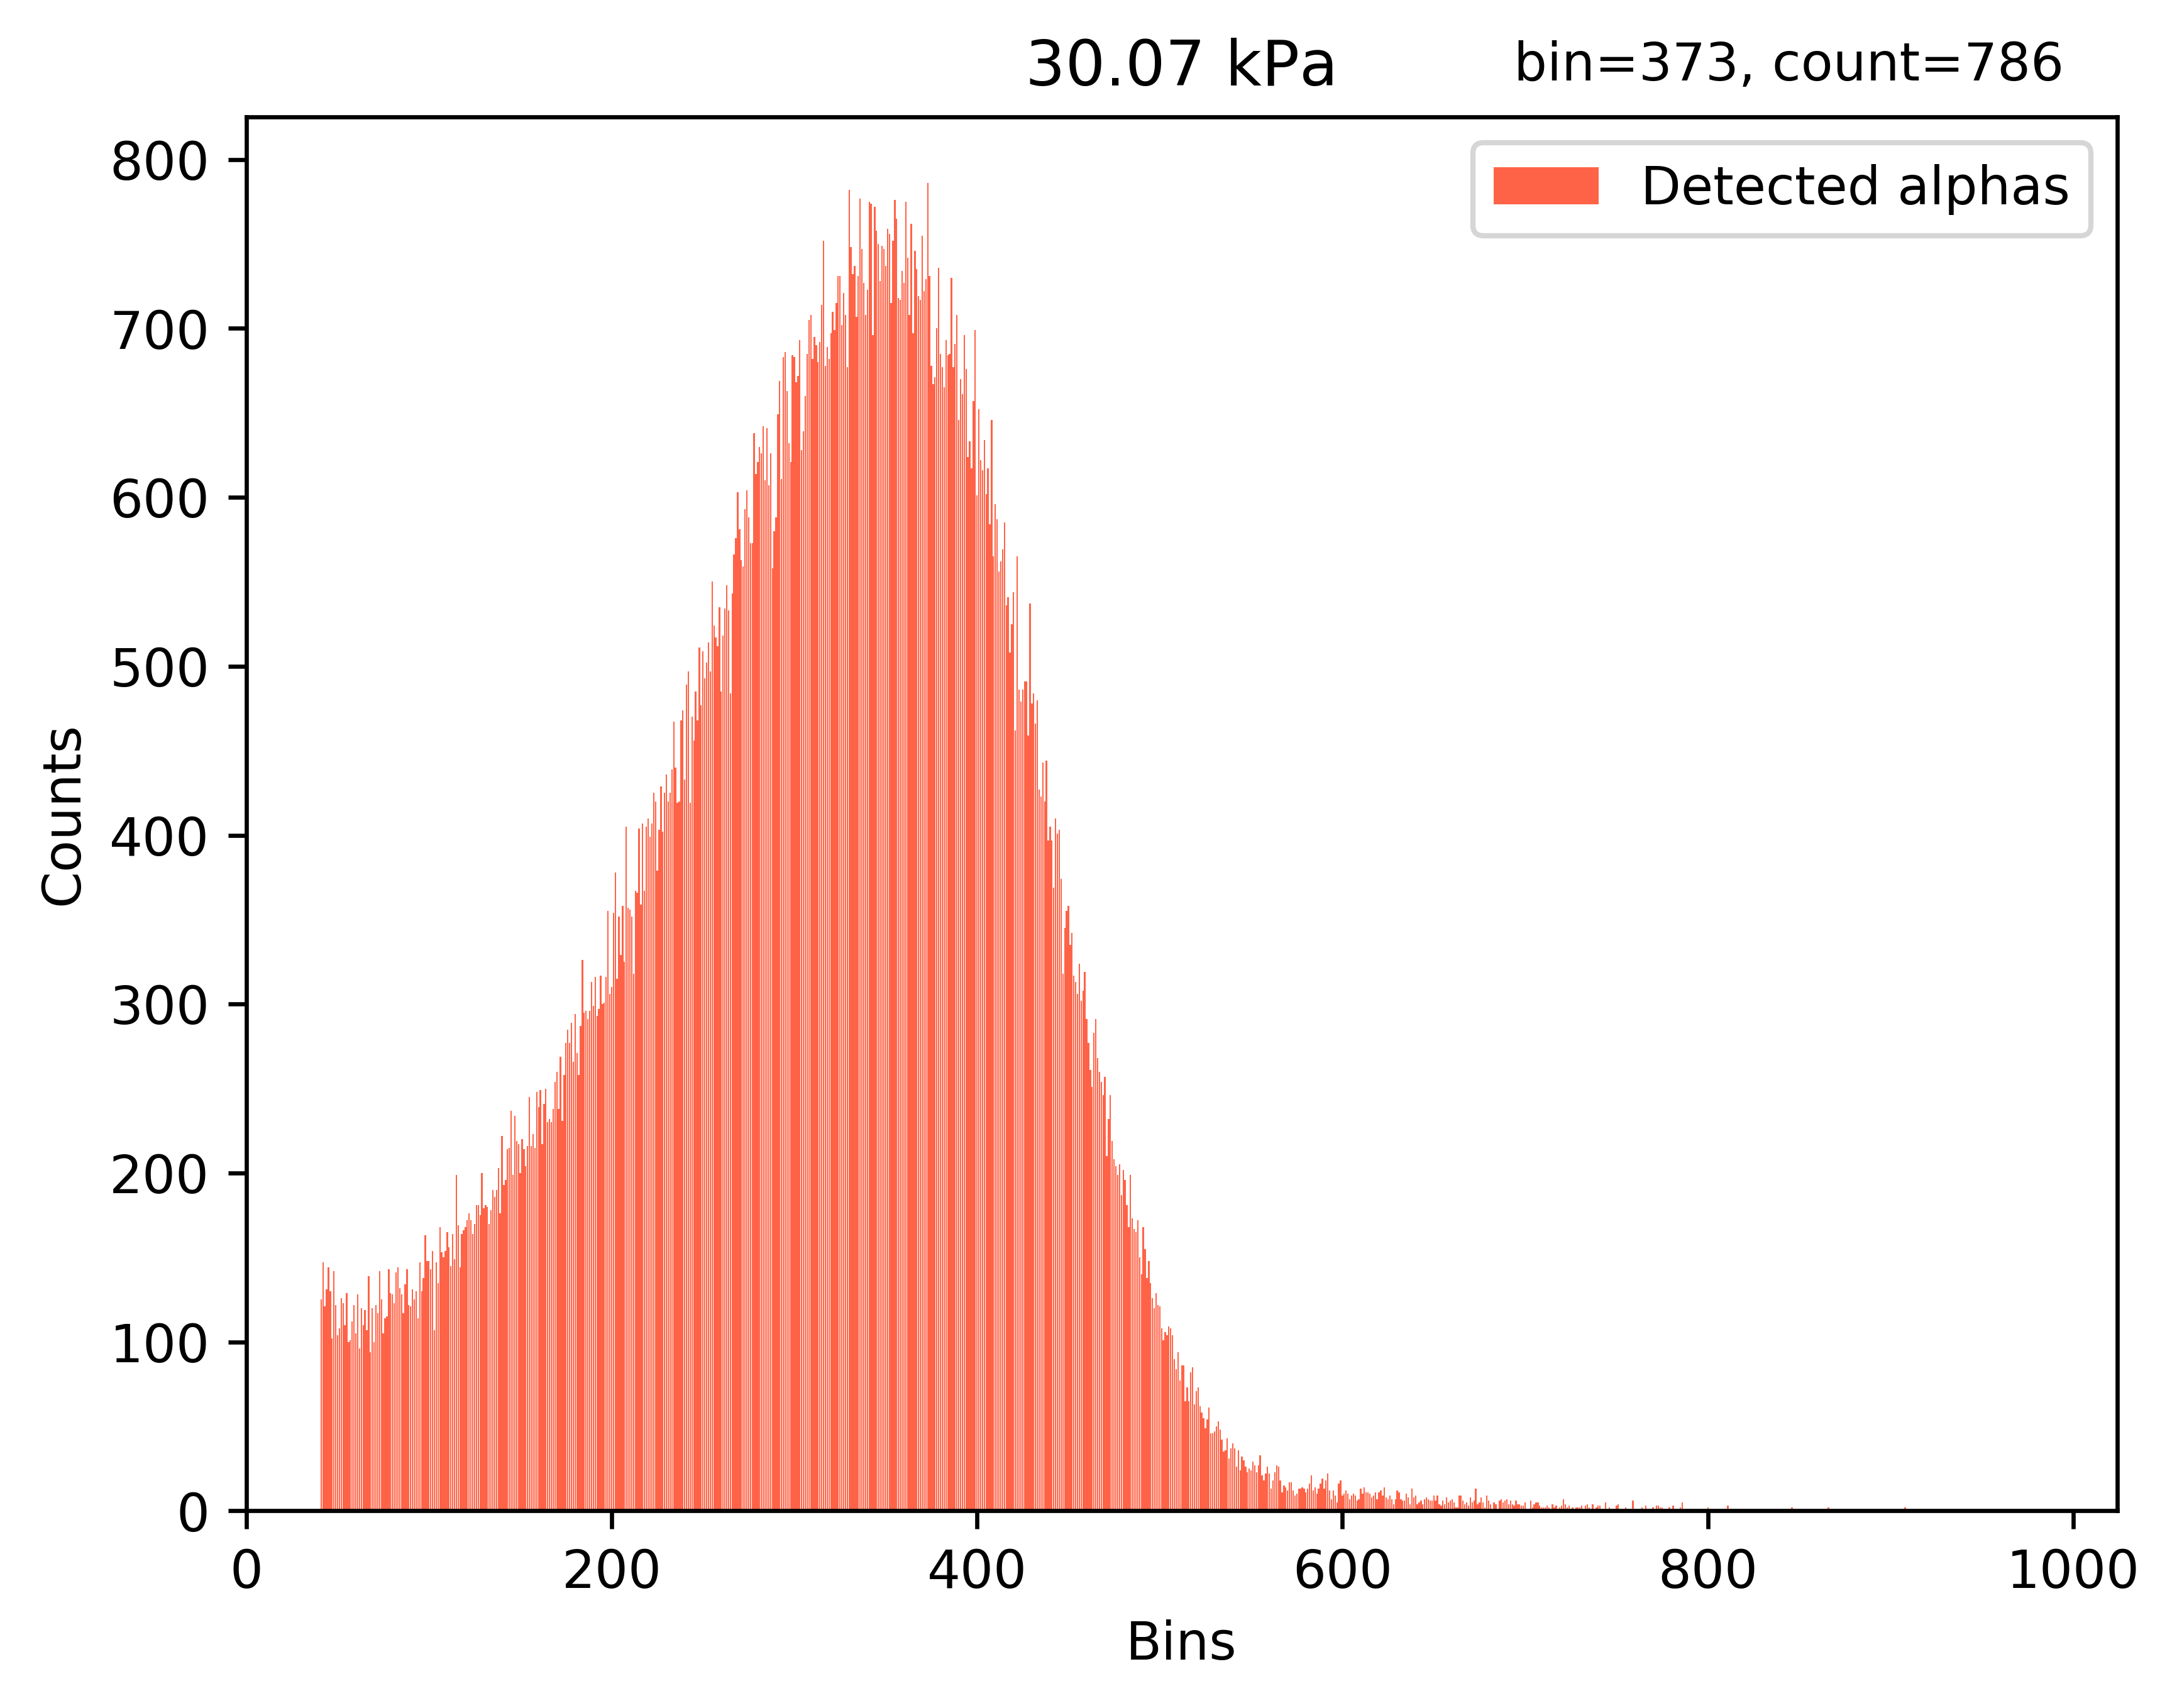
\includegraphics{raw_p=30.07kPa.png}
}}\\
\subfloat[]{\scalebox{0.37}{
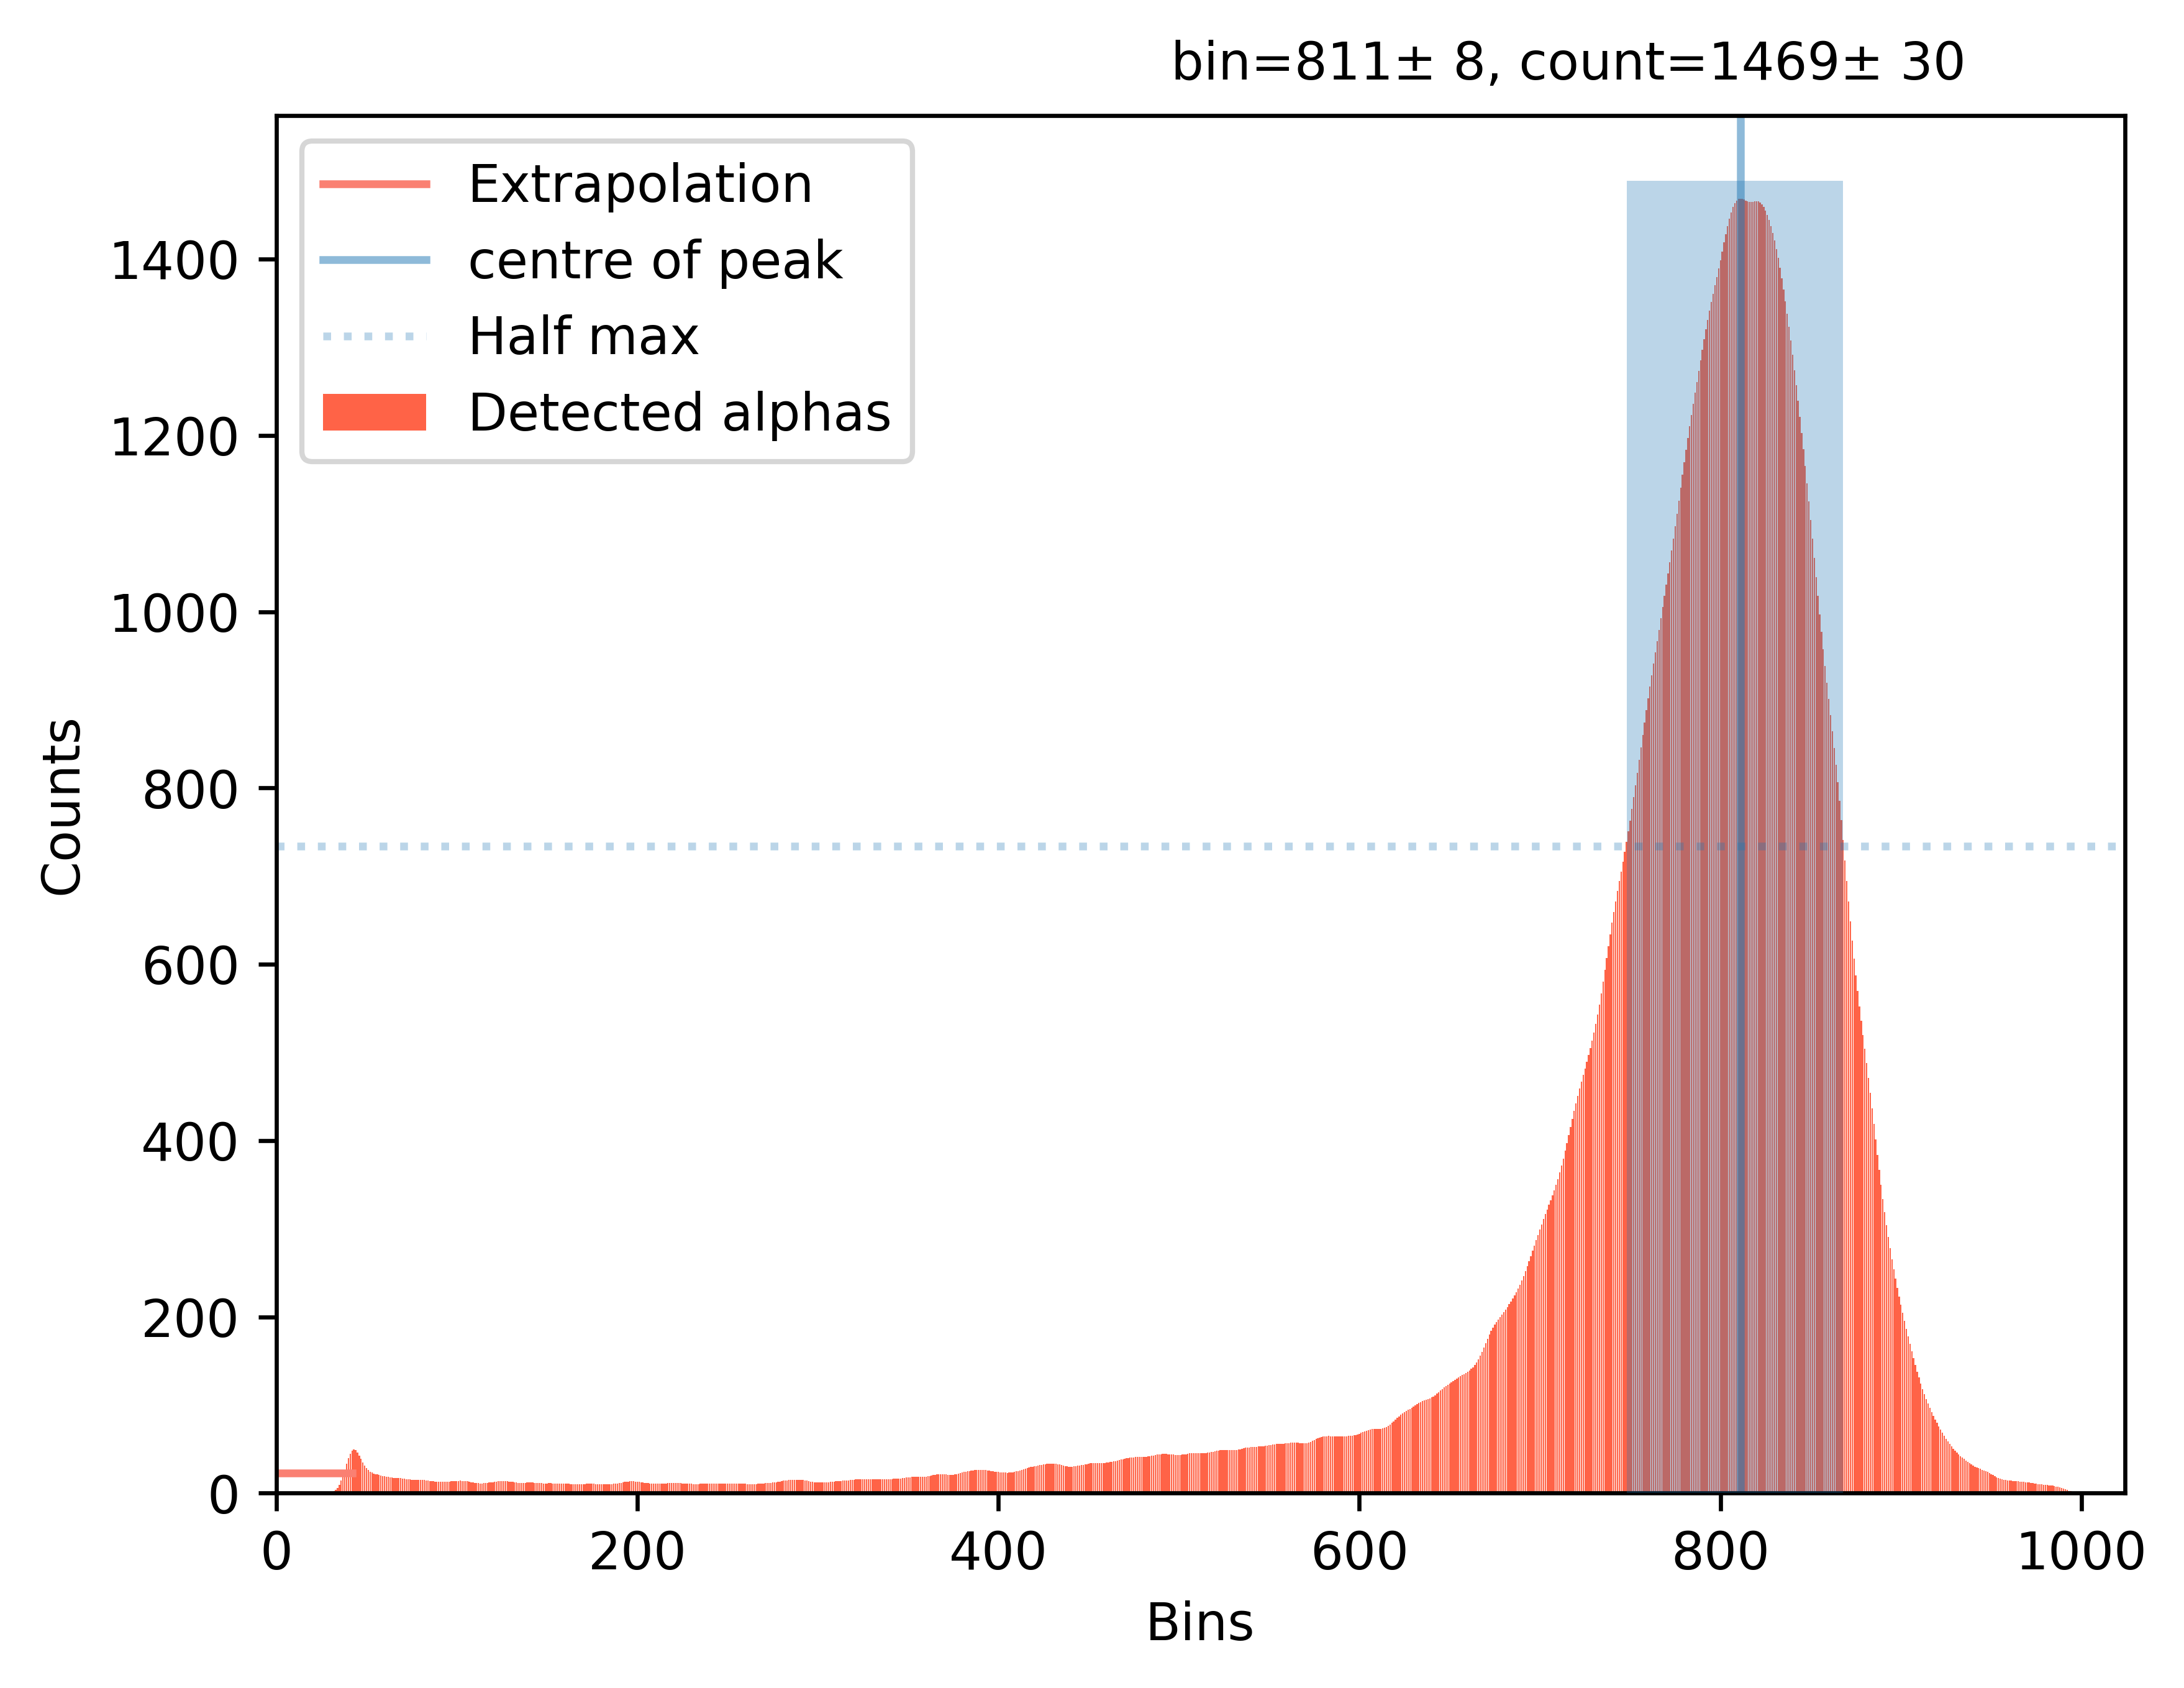
\includegraphics{smooth_p=5.17kPa.png}
}}
\subfloat[]{\scalebox{0.37}{
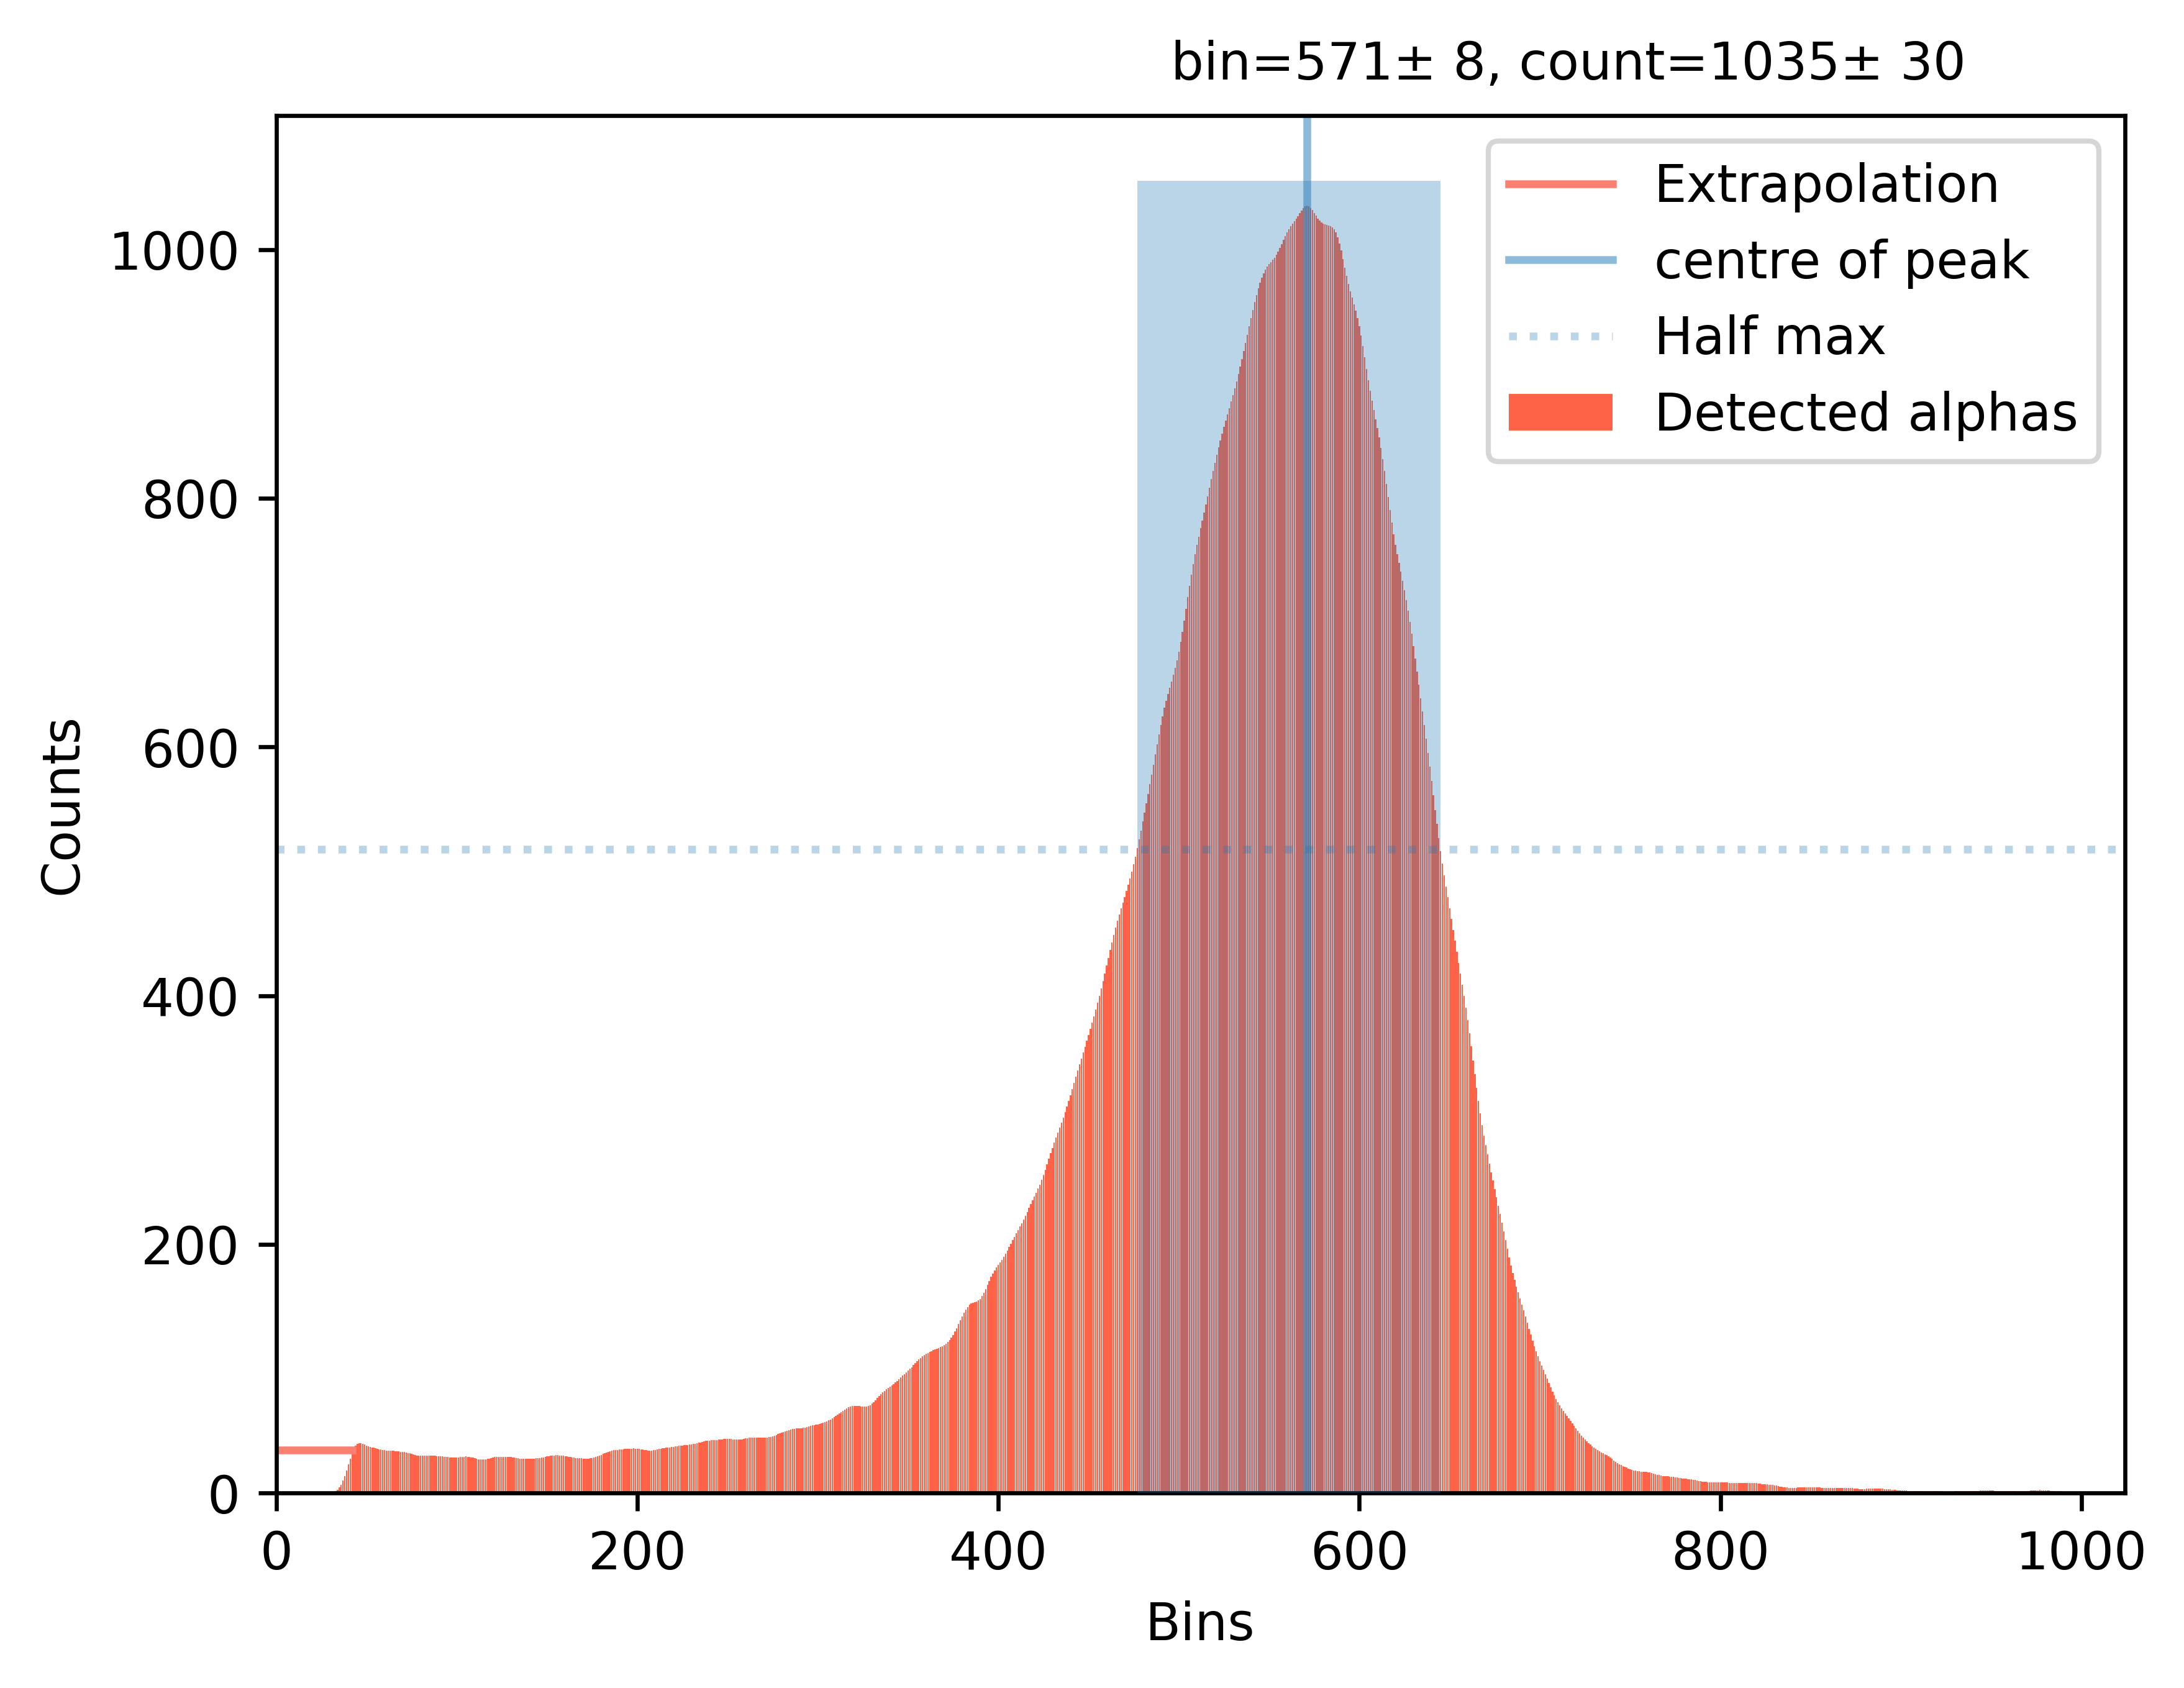
\includegraphics{smooth_p=19.97kPa.png}   
}}
\subfloat[]{\scalebox{0.37}{
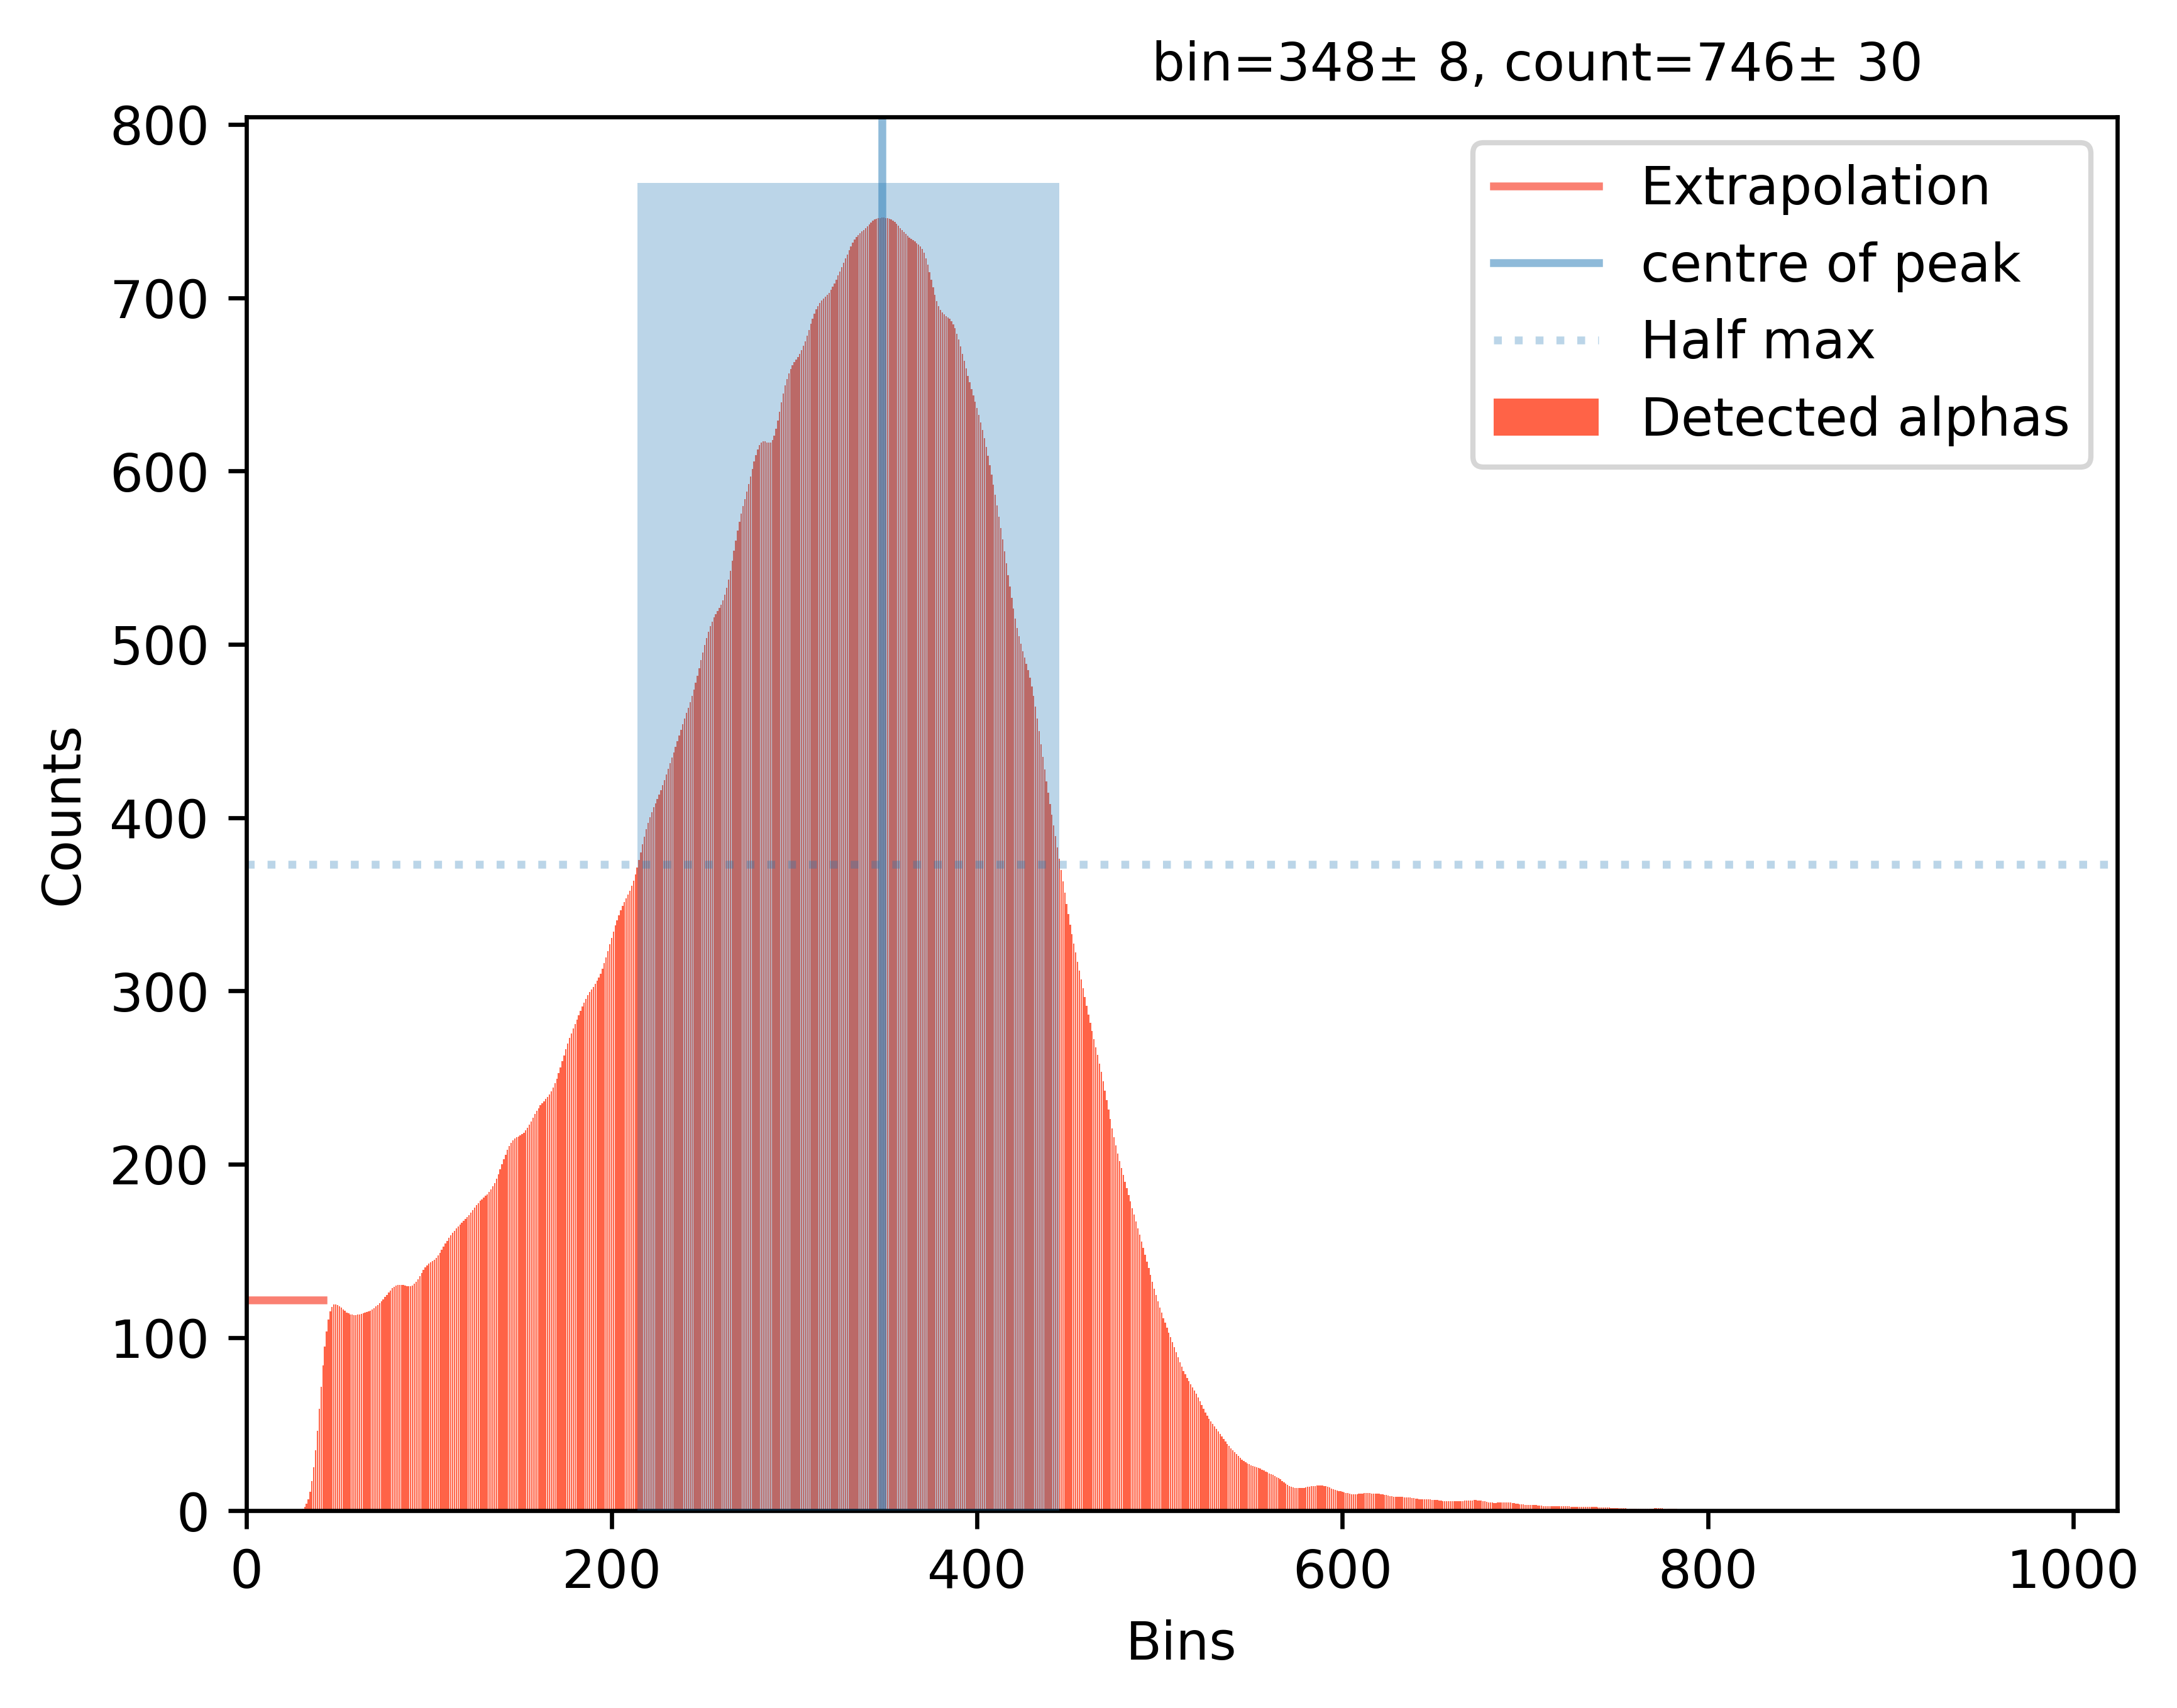
\includegraphics{smooth_p=30.07kPa.png}
}}
\caption{These 6 spectra serve as an example of unprocessed and processed spectra for alpha particle ranges. Spectra (a),(b),(c) are the raw data. Spectra (d),(e),(f) have been processed using "gaussian smoothing". The corresponding pressure values are 5.17 kPa, 19.97 kPa and 30.07 kPa respectively. In addition to the data in the smoothed spectra plots, we have included an extrapolation for the region below the noise threshold. It can be observed (from left to right) that as pressure increases the whole spectrum of the detected alpha particles moves towards the low energy region.
}
\end{figure}
\clearpage
\begin{SCfigure}
\subfloat[]{\scalebox{0.5}{
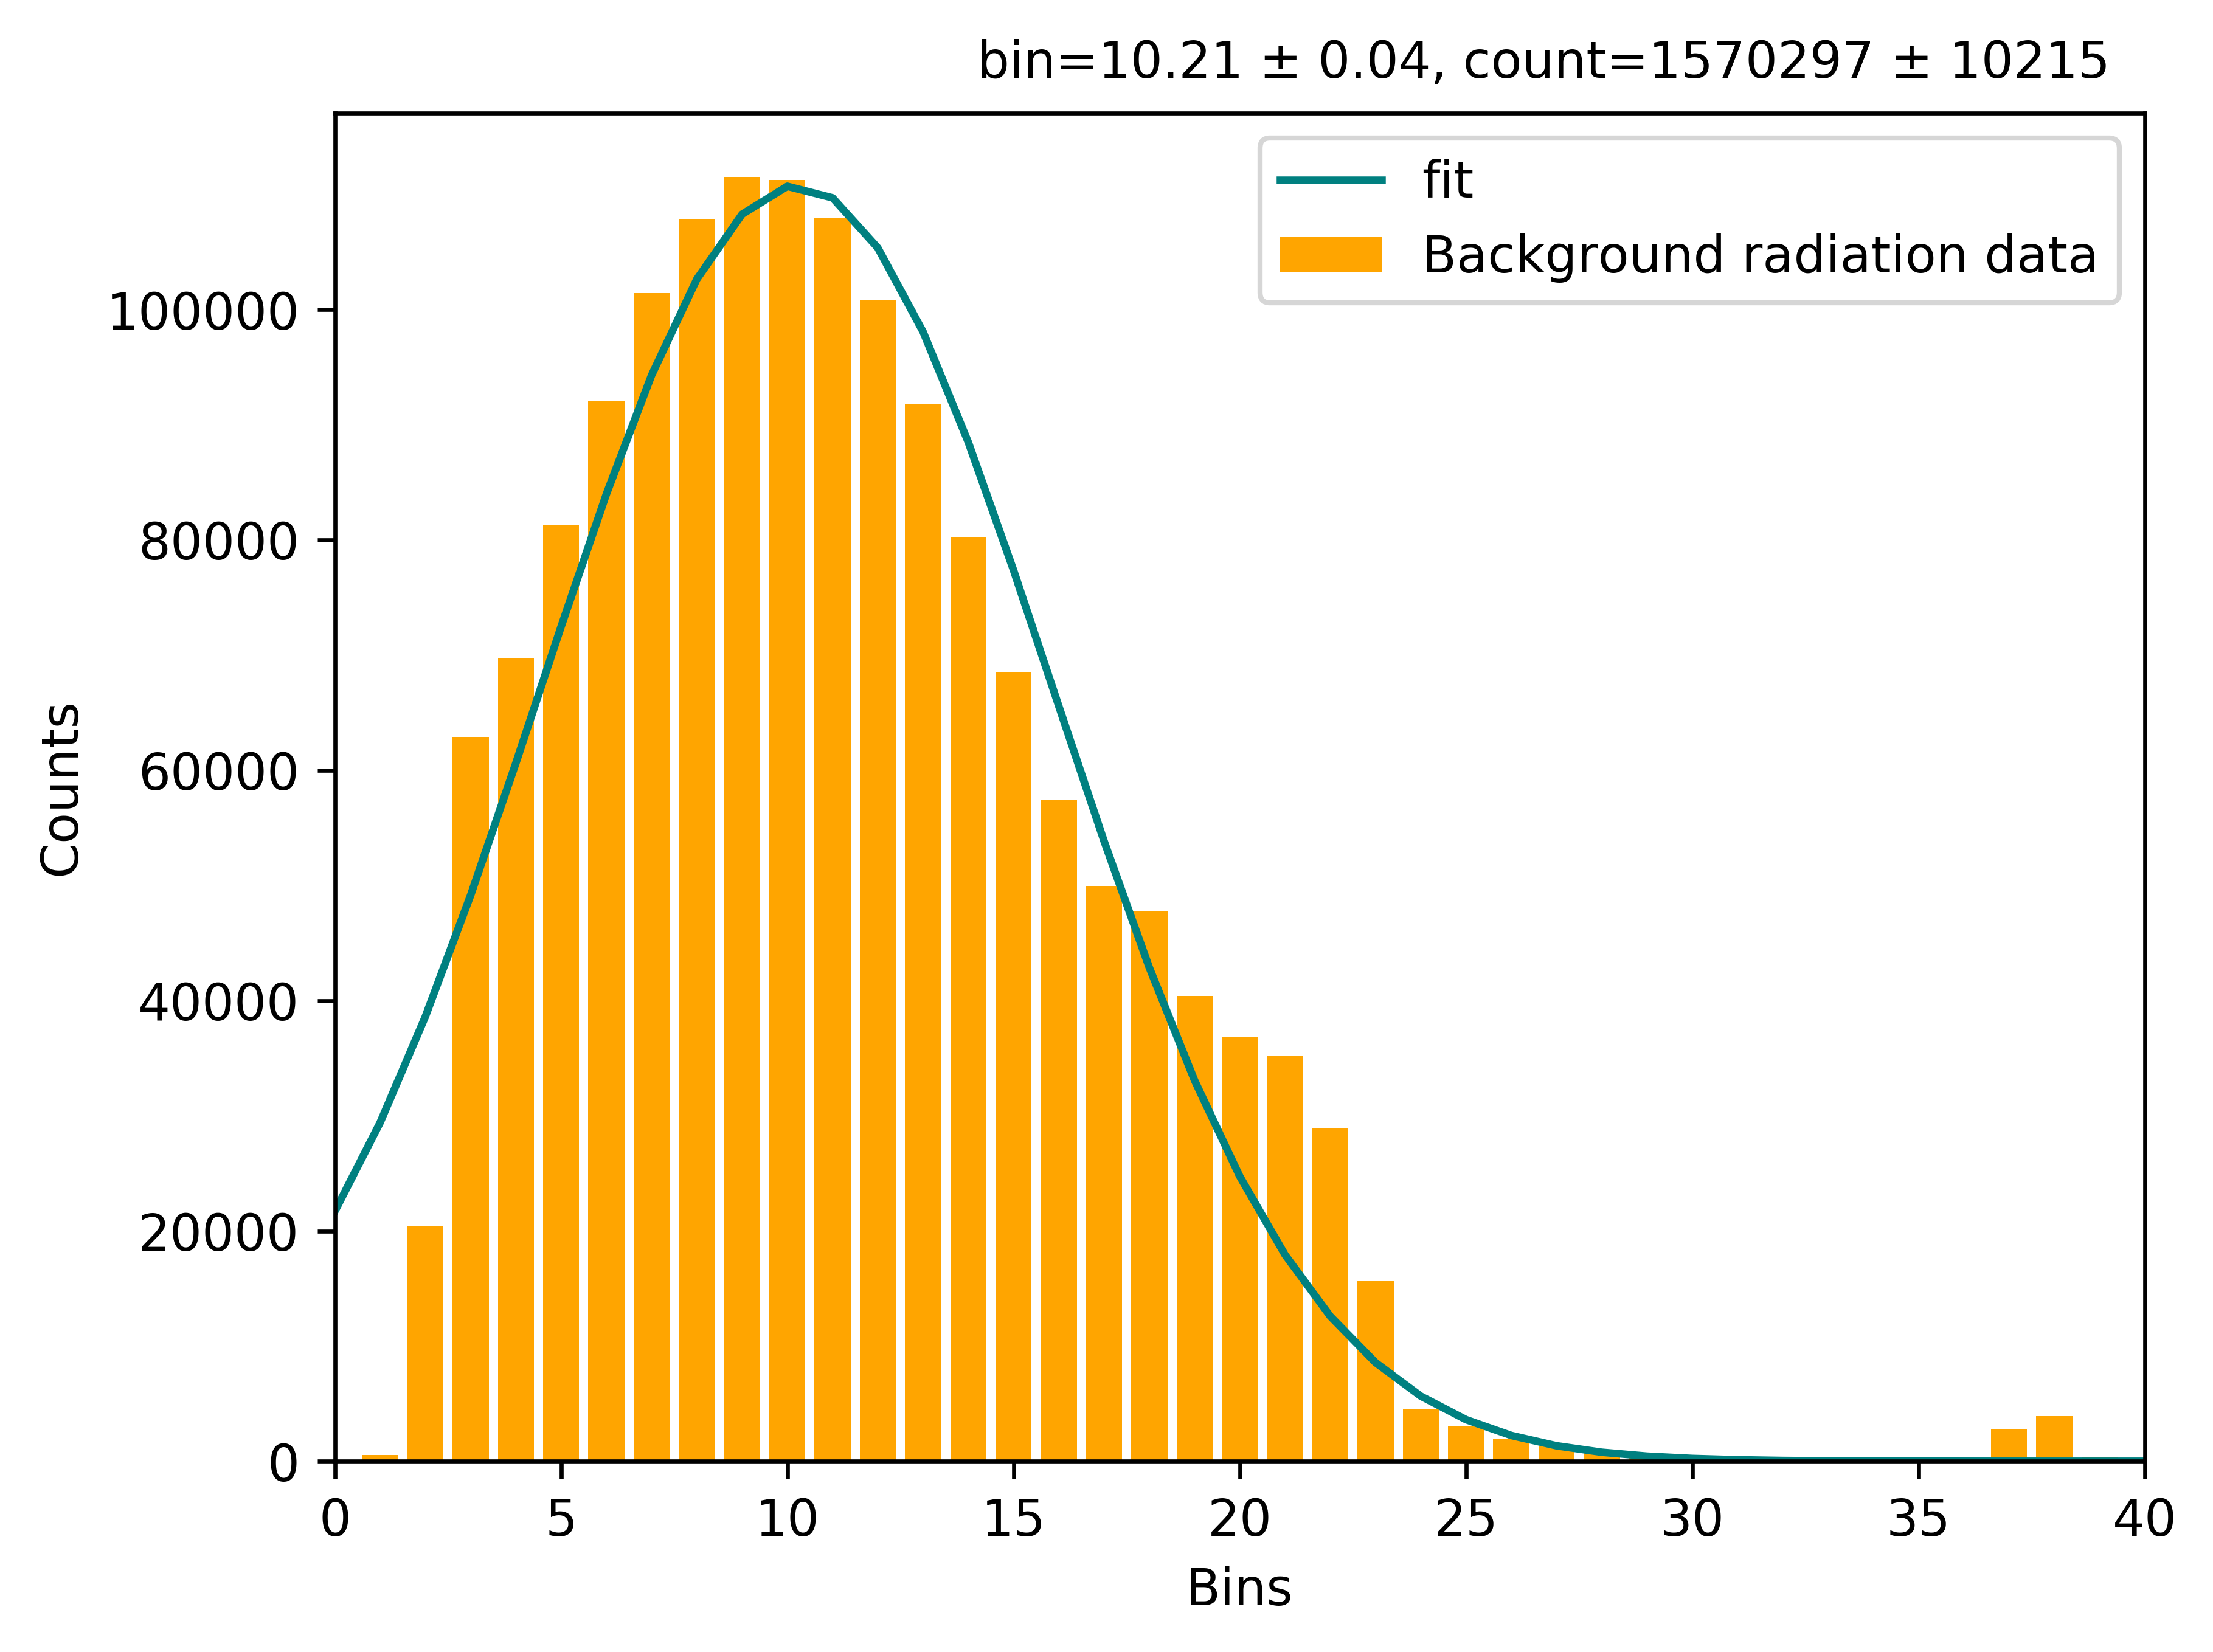
\includegraphics{background.png}
}}
\caption{
 We find the bin location corresponding to the zero energy using the background spectrum recorded with a threshold of 4 bins. The spectrum has been fit with a gaussian curve. From our fit we find the zero energy point (ie. the mean of the gaussian) this value is bin number $10.21 \pm 0.04$. We will use this value in all subsequent analysis, since our each of our spectra need to be corrected by this offset.
 }
\end{SCfigure}
\clearpage

%-----------------------------------------------------------------------------------------
From the Brag--Kleeman rule, we find the anticipated range $R$ for the alpha particles passing through a thick gold sample $R = (6.0 \pm 0.2)\mu$m.

From equation (13) we calculate the thickness of the gold coating on the source construction $\Delta x = 2.45 \pm 0.08\mu$m. The difference between our calculated thickness of the gold layer of the source construction and the reported thickness by the manufacturer\cite{SPA} ($3 \mu$m) is $ = 0.55 ± 0.08\mu$m.
%-----------------------------------------------------------------------------------------

\begin{SCfigure}
\subfloat[]{\scalebox{0.5}{
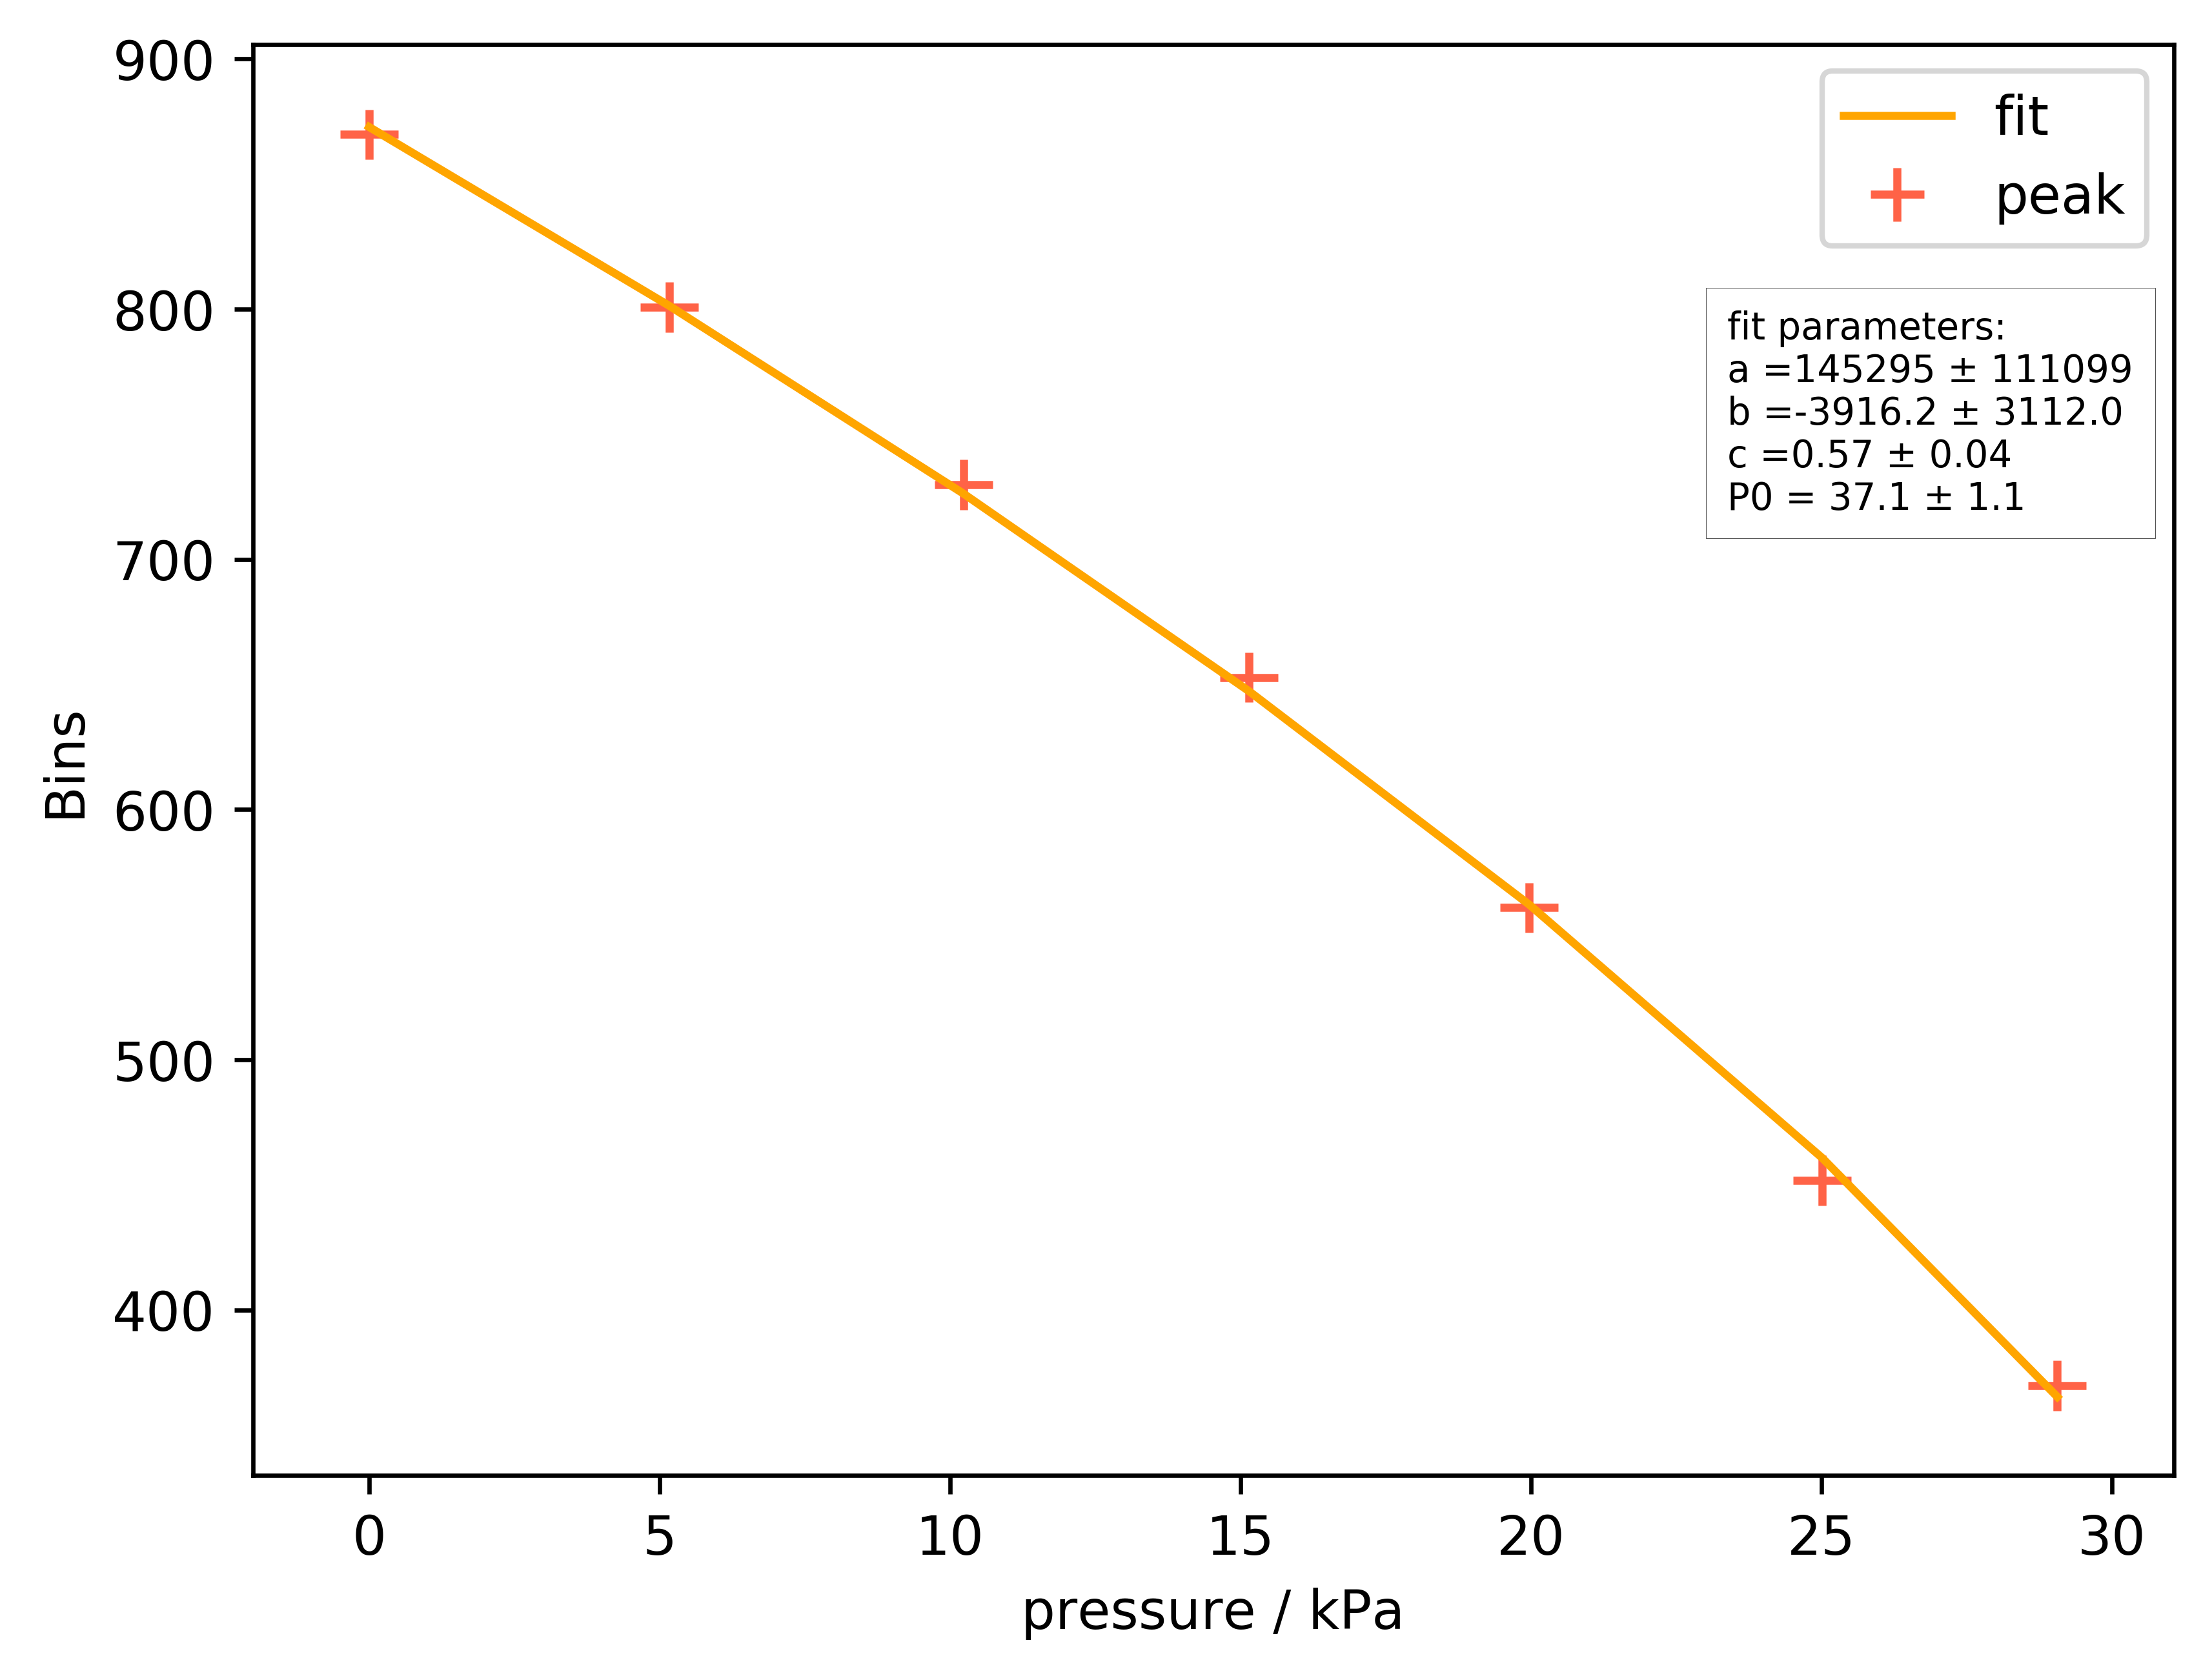
\includegraphics{peak_position_vs_pressure.png}
}}
\caption{
Using our smoothed spectra, we determined the pressure value $P_0$ corresponding to the absorption of alpha particles with the most probable energy, by making a power-law fit of the 6 highest energy peak values using the equation $y=(a+bp)^c$, where y is peak location, p is pressure\cite{feedback}. 
Firstly, We subtract the zero energy bin $10.21 \pm 0.04$ from all the peaks positions used in the fit. From our fit we find the pressure value $P_0 = 37.1 \pm 1.1$.
The fit parameter values are displayed in the figure. 
}
\end{SCfigure}

\begin{figure}[!htbp]
\subfloat[]{\scalebox{0.5}{
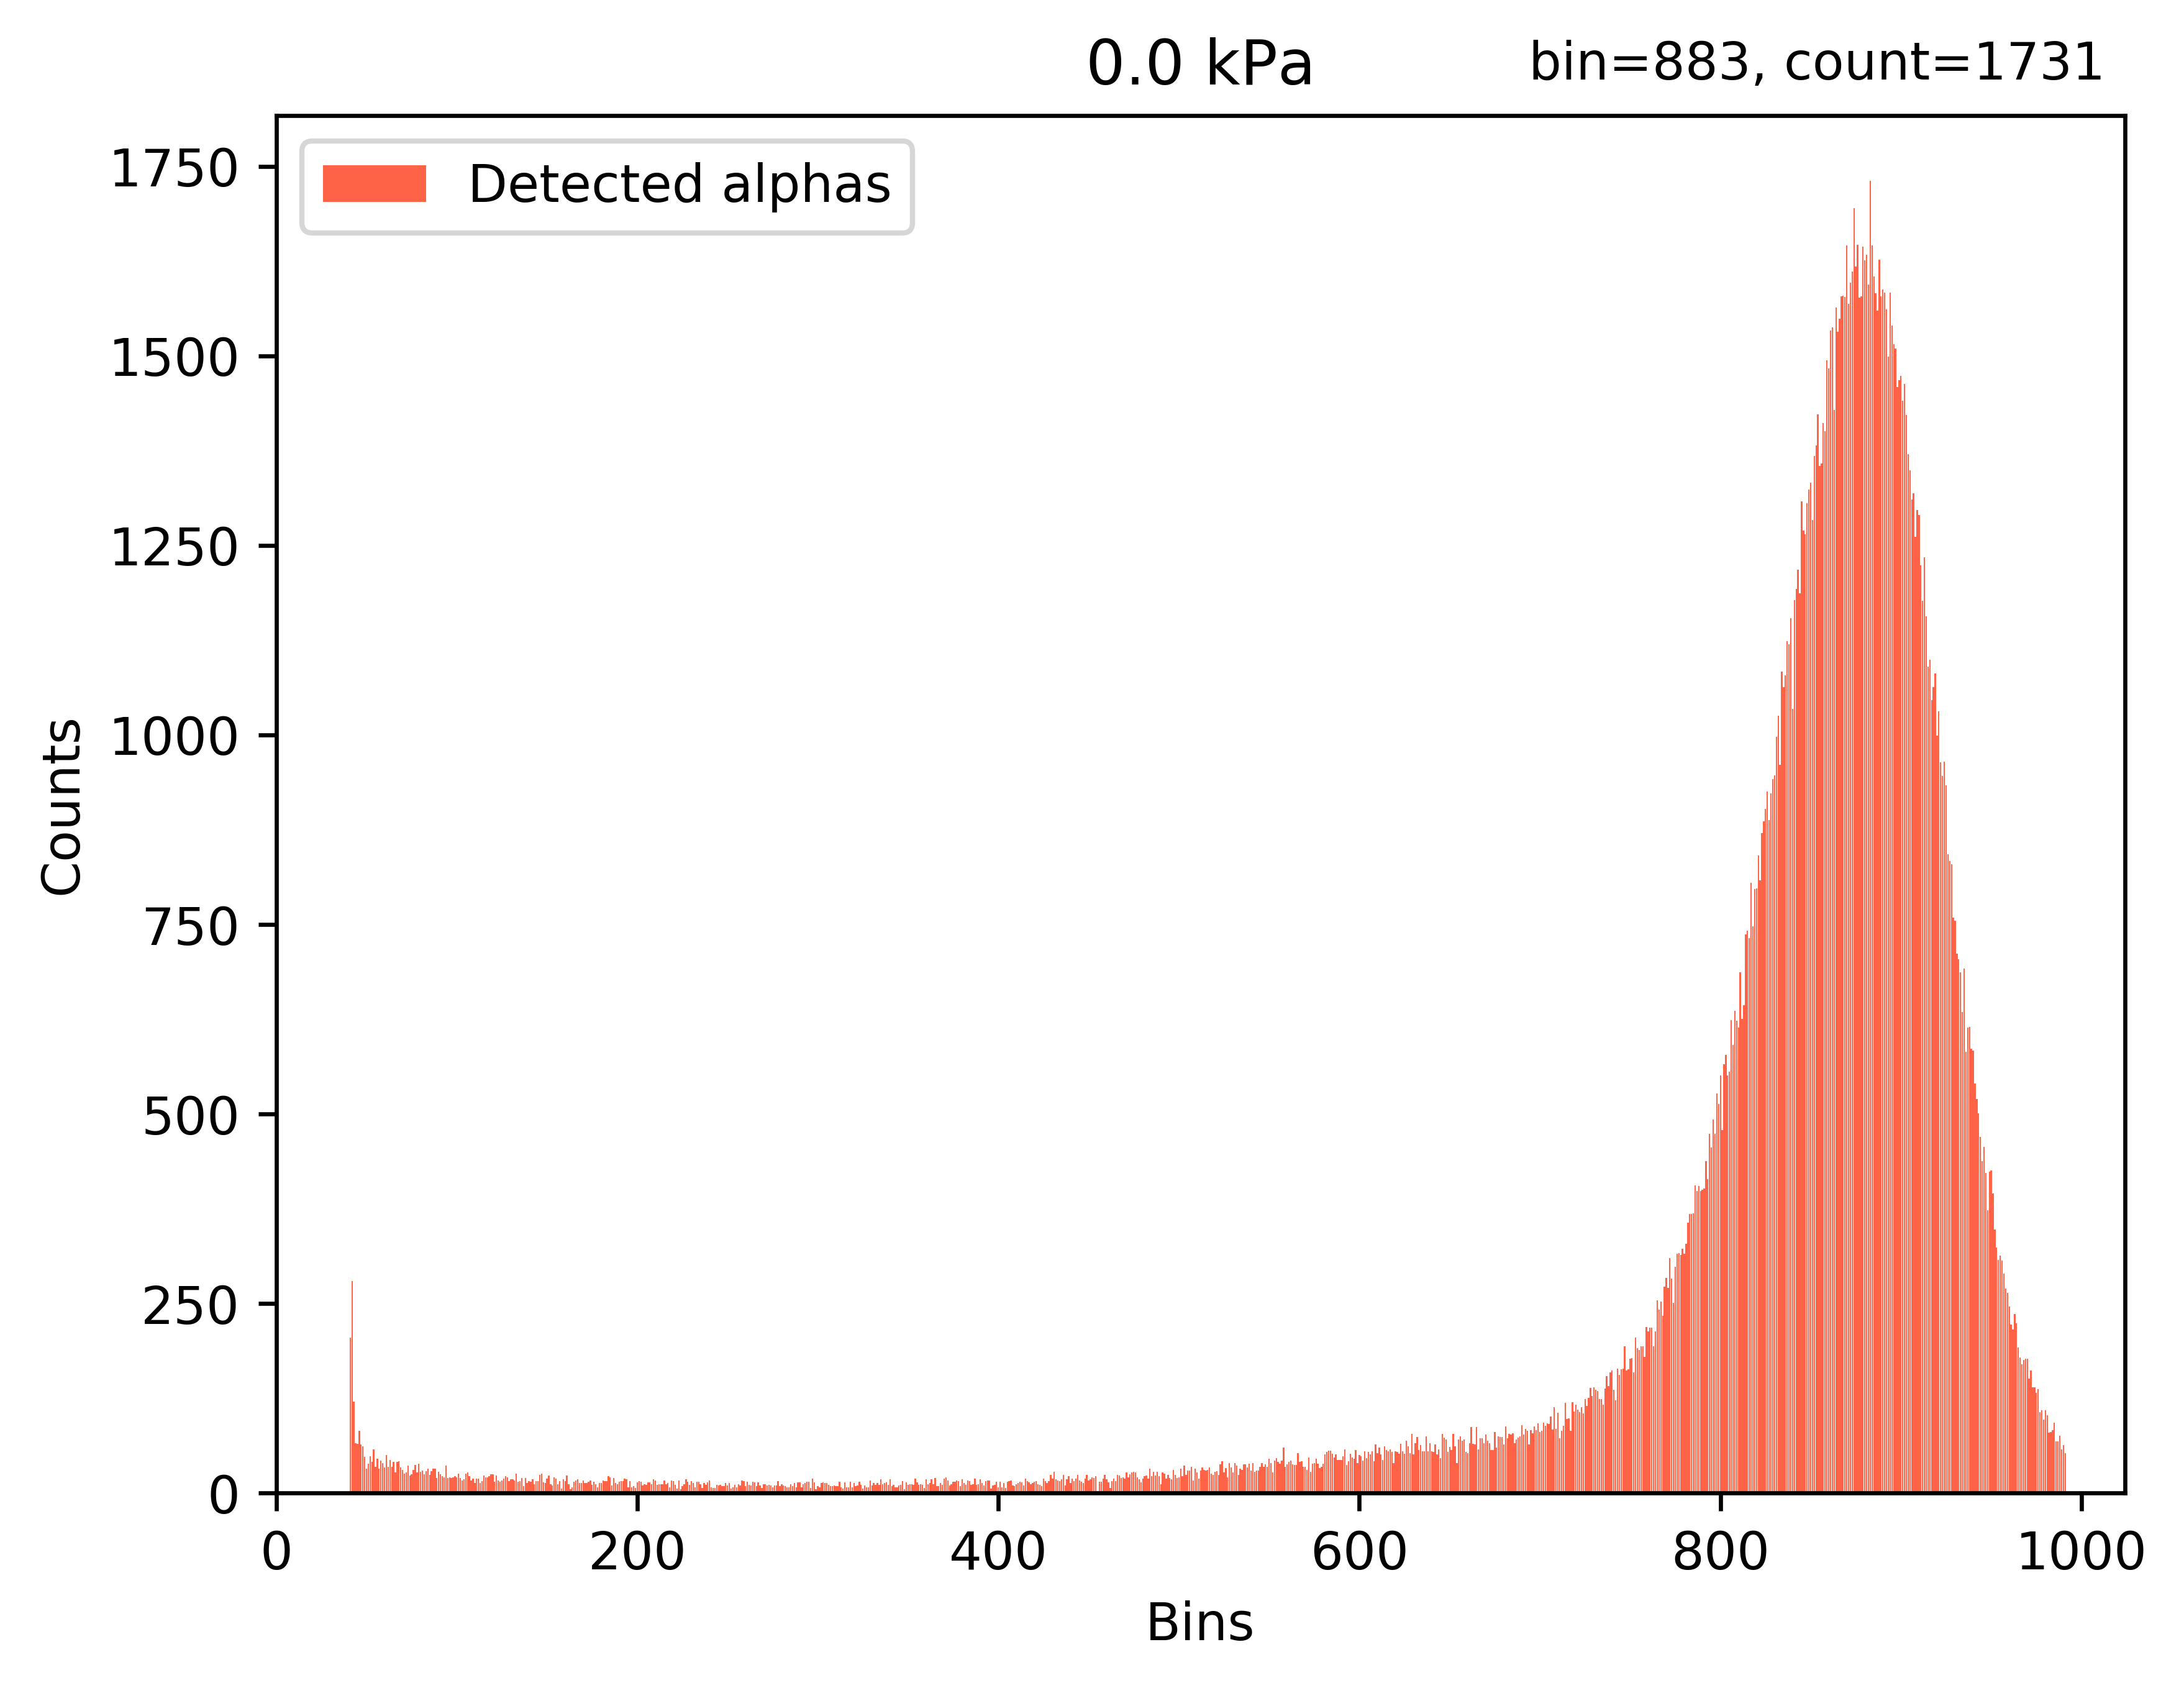
\includegraphics{raw_p=0.0kPa.png}    
}}
\subfloat[]{\scalebox{0.5}{
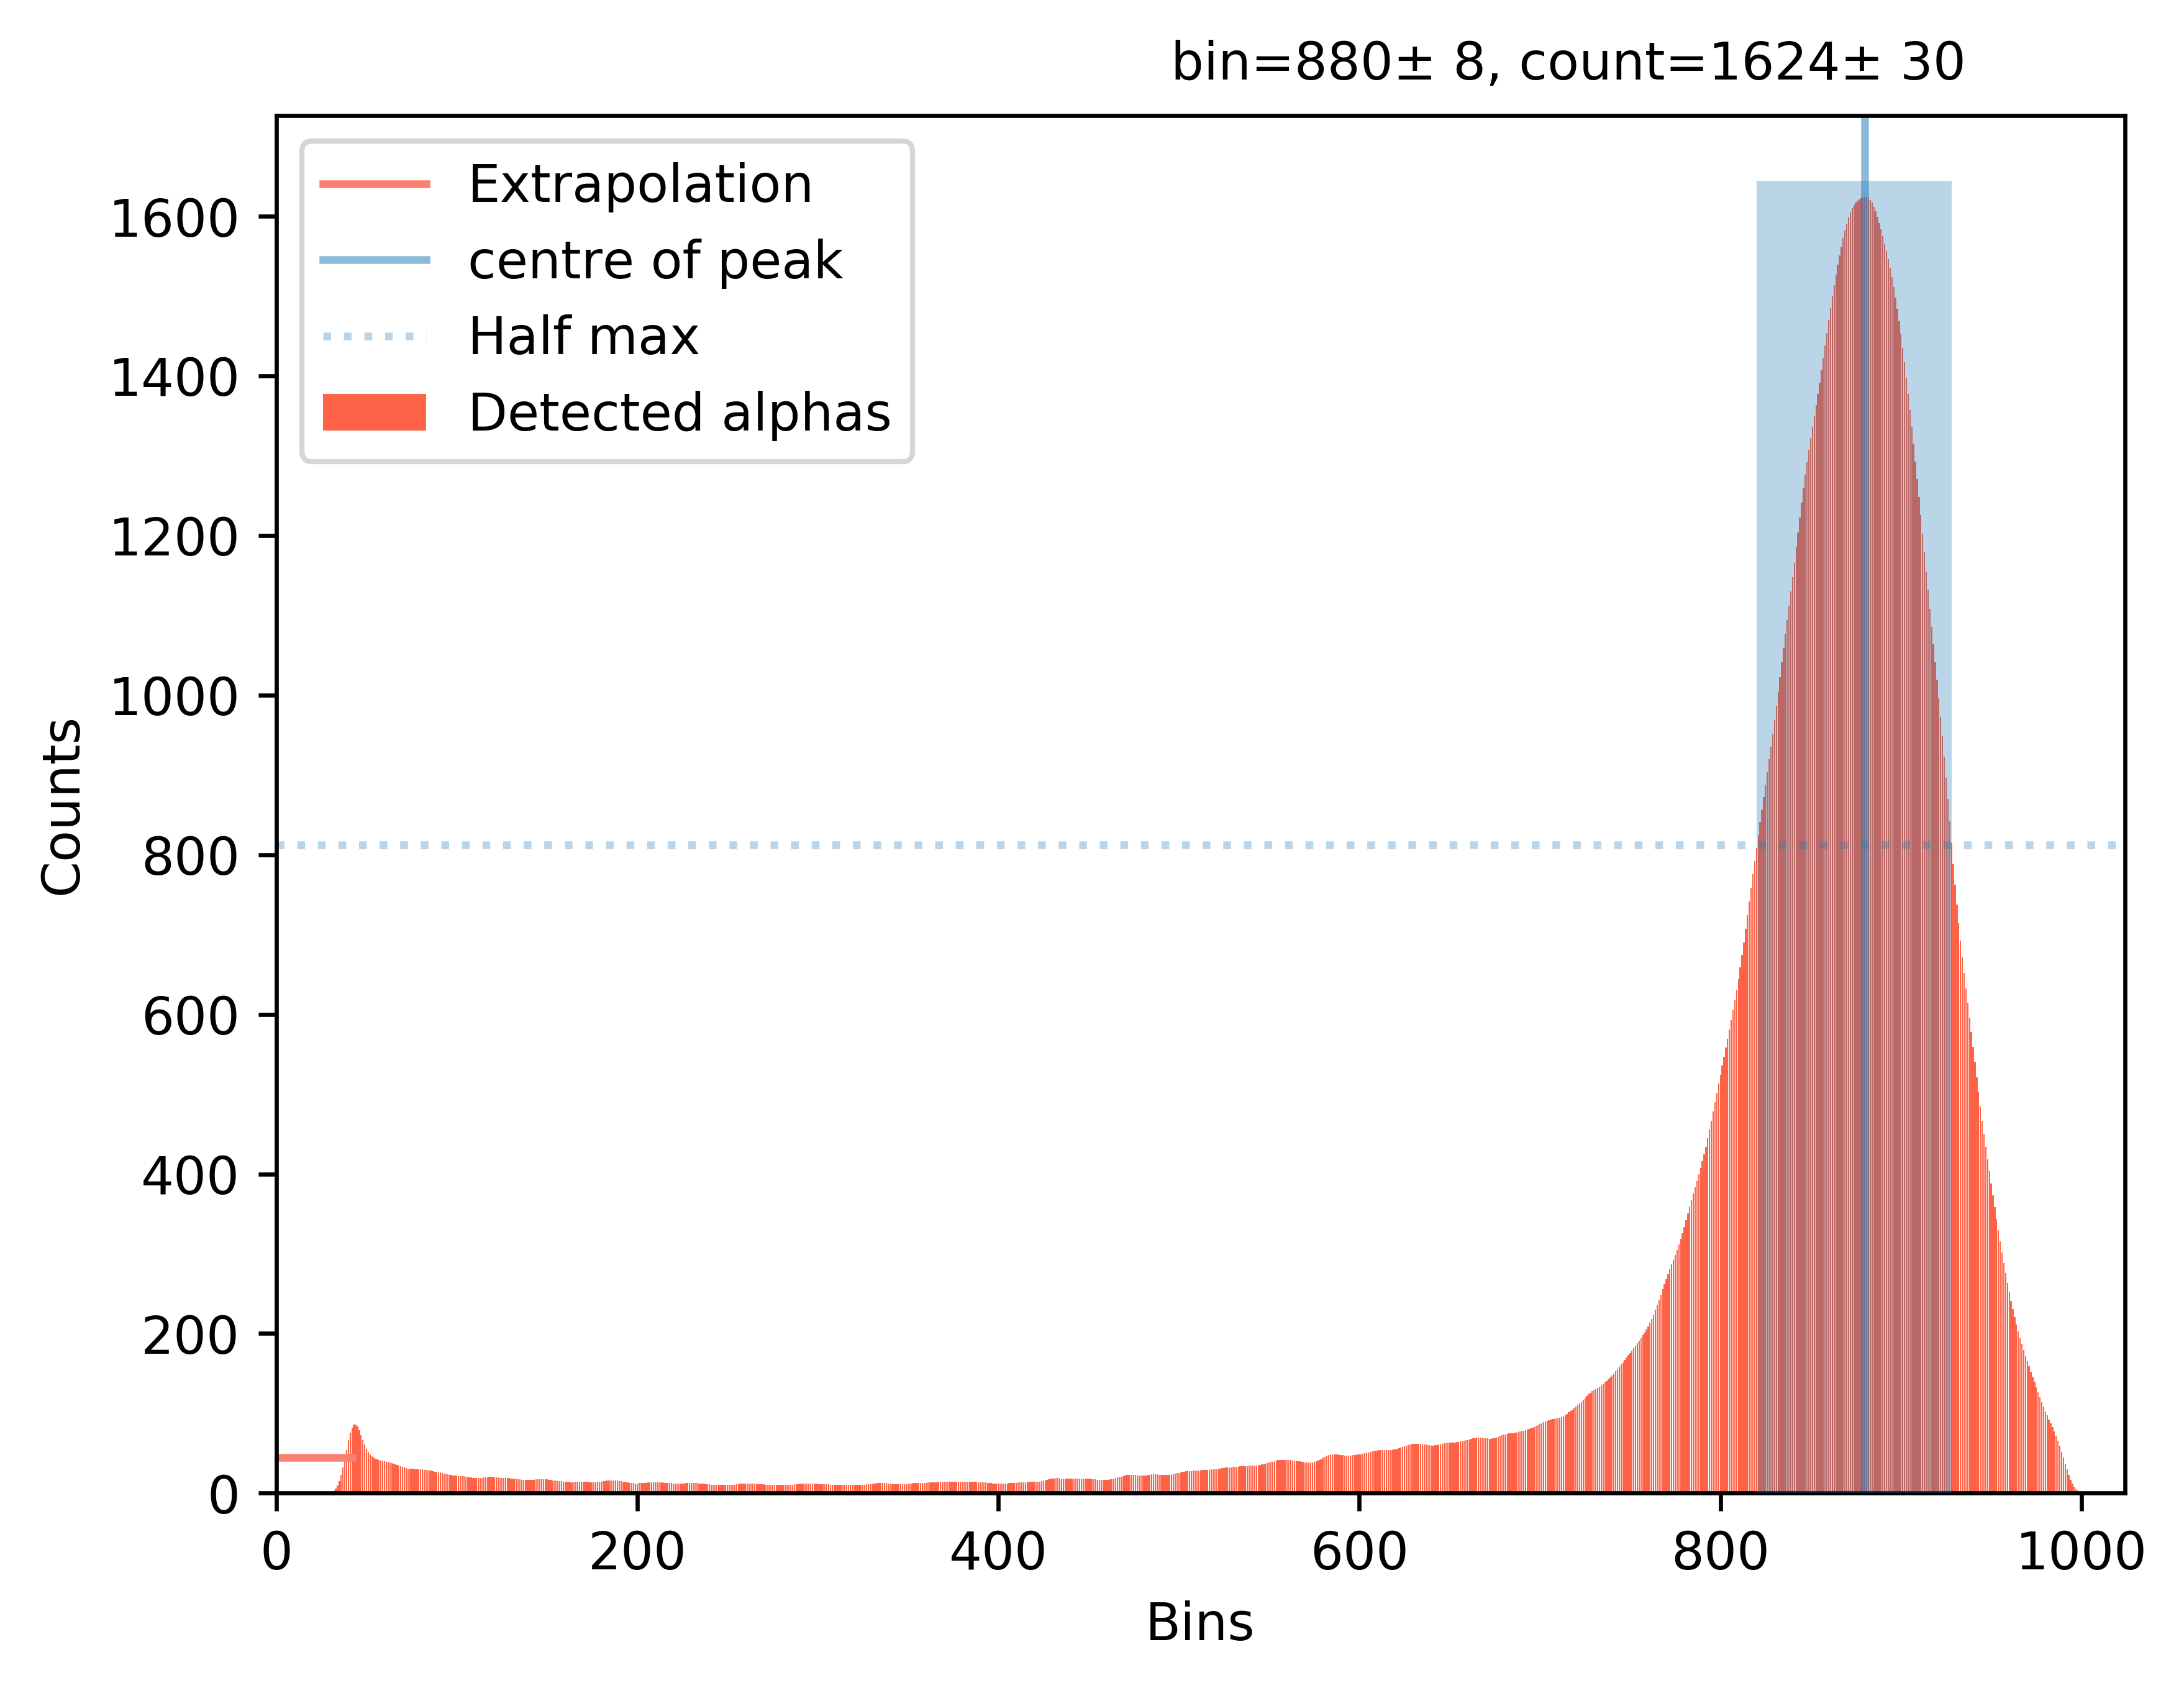
\includegraphics{smooth_p=0.0kPa.png}   
}}
\caption{
Using equation (6), we determine the alpha particle mass-energy (as the particles are emitted from the source) to be $E_0 = 4.46 \pm 0.09$ MeV. We compare the result to the energy emitted from \textsuperscript{241}Am\cite{SPA} $E = 5.4857$ MeV. The difference in these values is $1.03 \pm 0.09$ MeV.
To determine the calibration factor for the MCA in terms of the energy, we calculate the calibration factor $1$bin$ = 5.1 \pm 0.1$keV. To do this we divide the value of $E_0$ by its corresponding bin in figure (b) minus the zero point energy bin.
}
\end{figure}


\clearpage
% %-----------------------------------------------------------------------------------------
% From the Brag--Kleeman rule, we find the anticipated range $R$ for the alpha particles passing through a thick gold sample $R = (6.0 \pm 0.2)\mu$m.

% From equation (13) we calculate the thickness of the gold coating on the source construction $\Delta x = 2.45 \pm 0.08\mu$m. The difference between the calculated thickness of gold layer of the source construction and the reported thickness by the manufacturer ($3 \mu$m) \cite{SPA} is $ = 0.55 ± 0.08\mu$m.
% %-----------------------------------------------------------------------------------------


\begin{SCfigure}
\subfloat[]{\scalebox{0.5}{
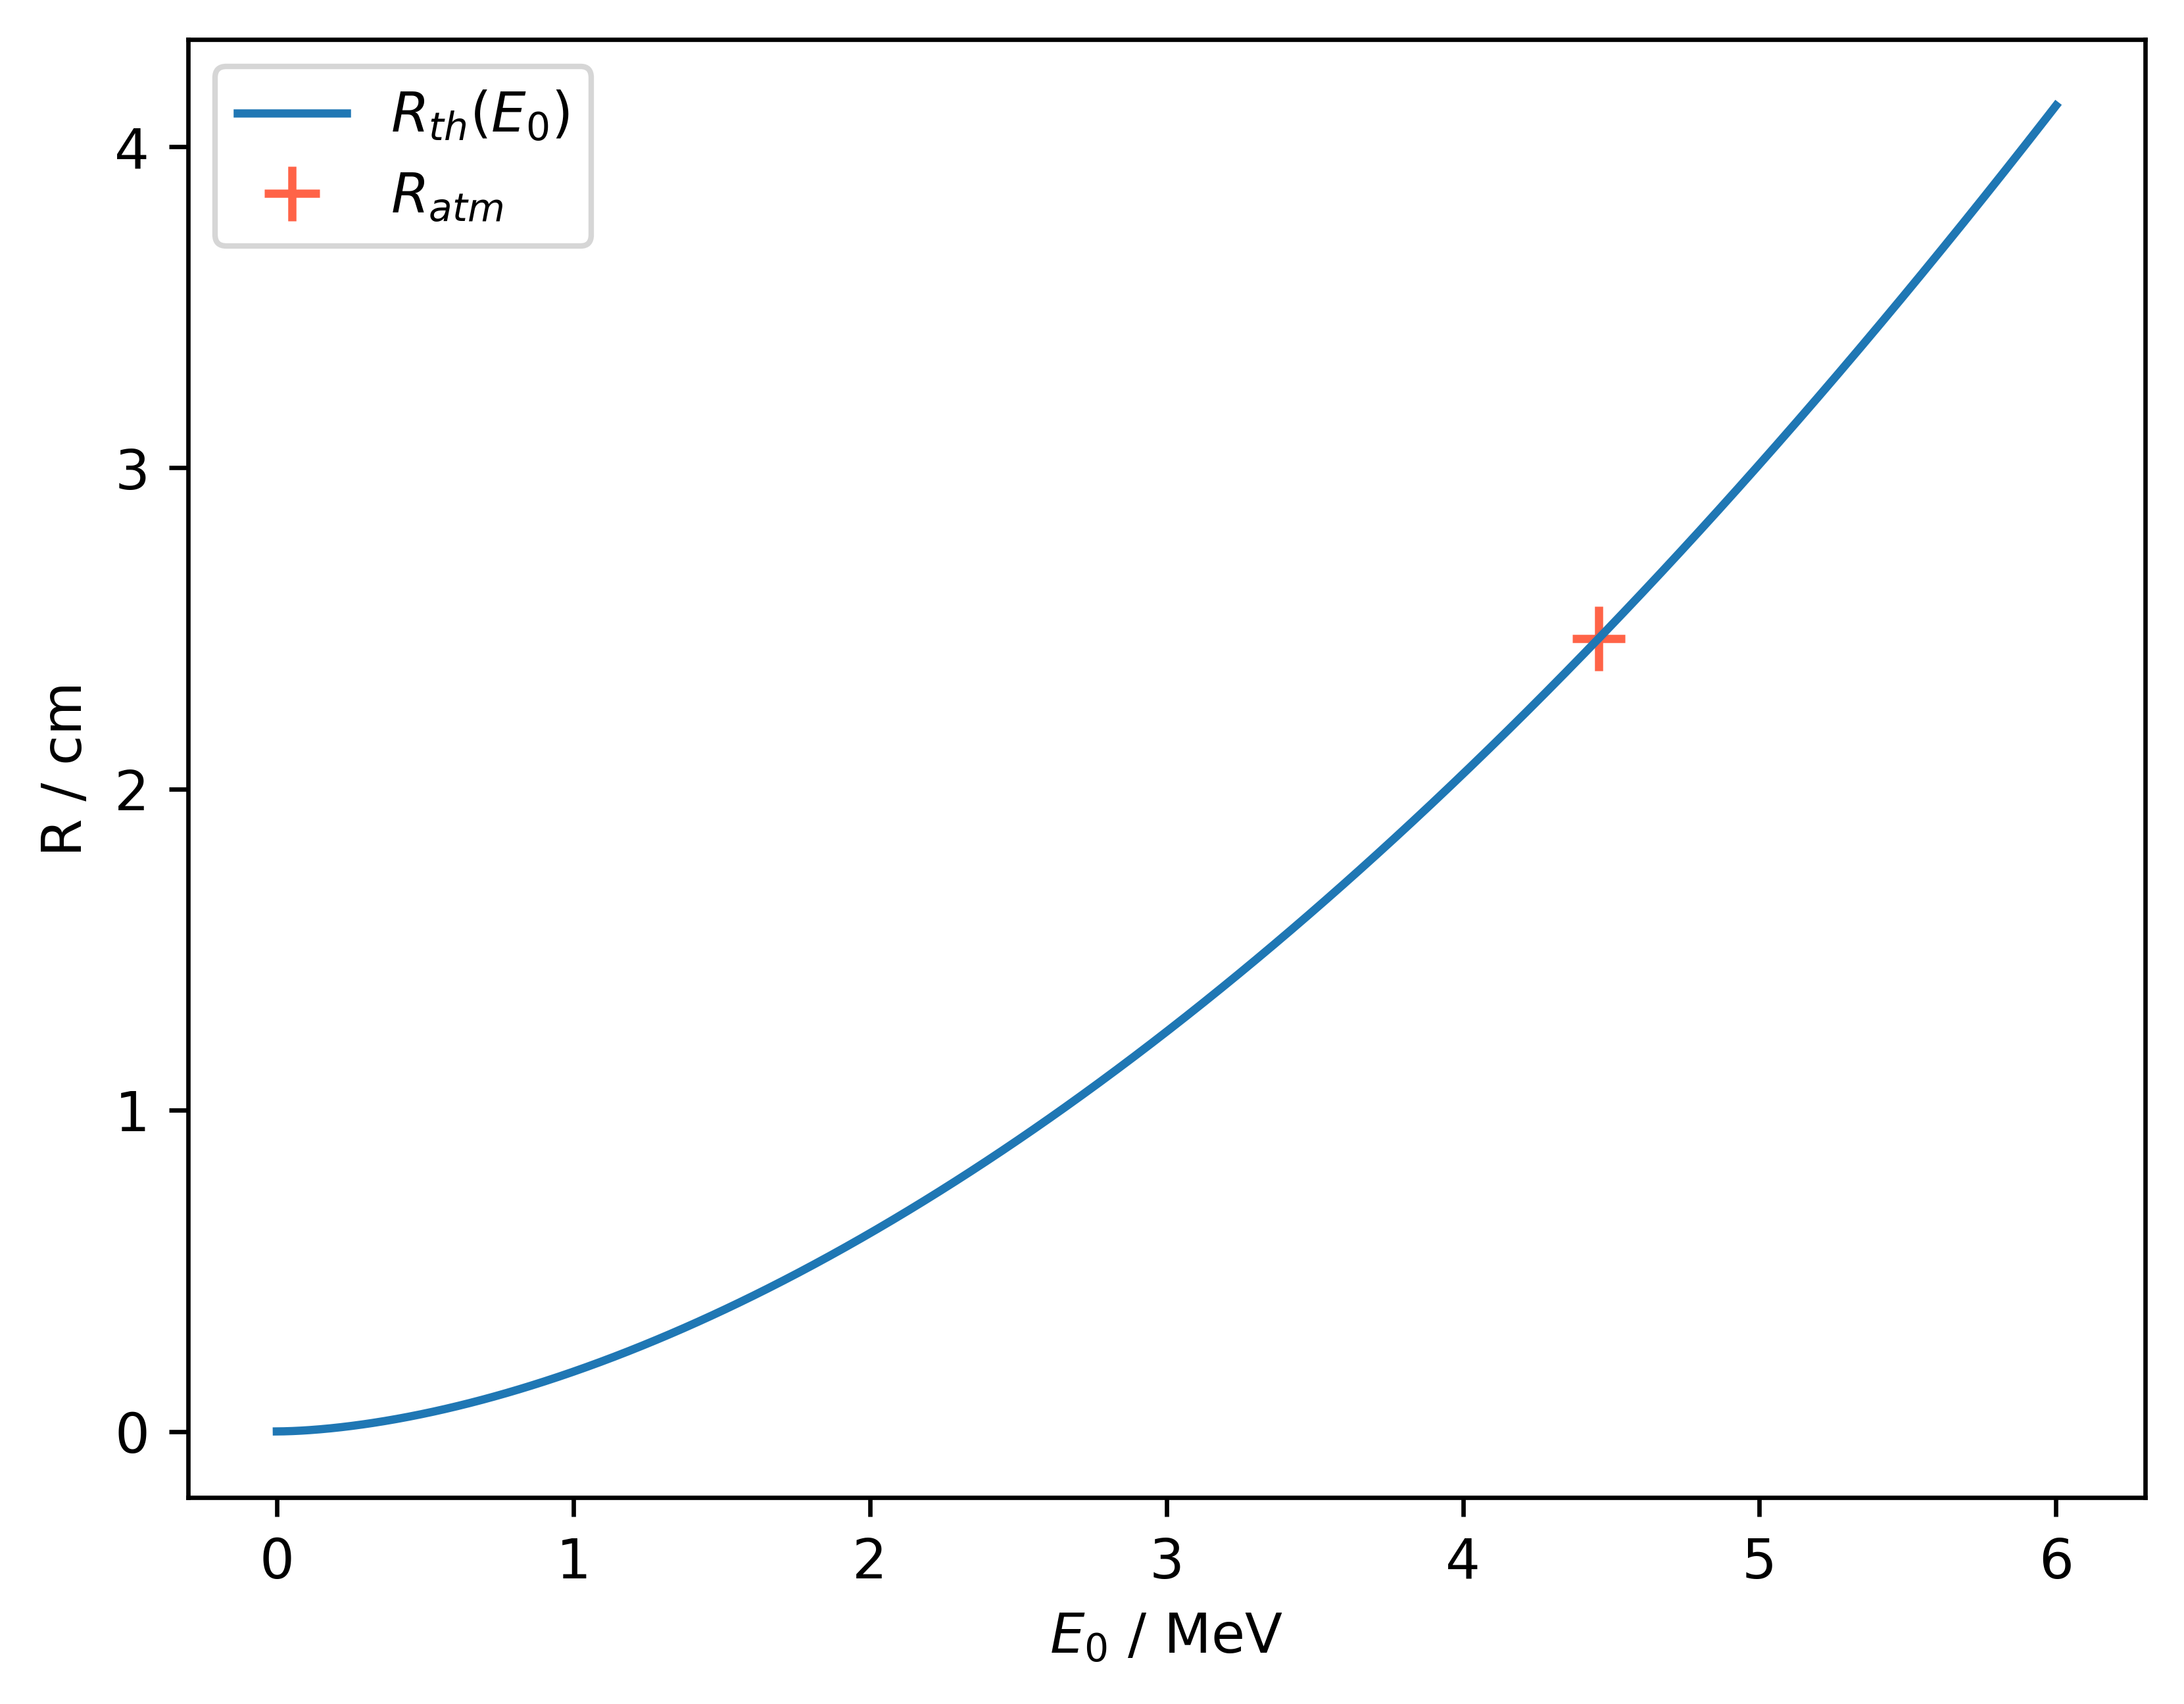
\includegraphics{theoretical_R_vs_E.png}
}}
\caption{Theoretical range of alpha particles in air as a function of their initial mass-energy $(E_0)$. The initial alpha particle energies are in the range from 0 to 6 MeV. We included the theoretical range point for atmospheric pressure conditions, $R_{atm} = 2.47 \pm 0.08$cm, calculated from equation (3).
}
\end{SCfigure}

\begin{SCfigure}
\subfloat[]{\scalebox{0.5}{
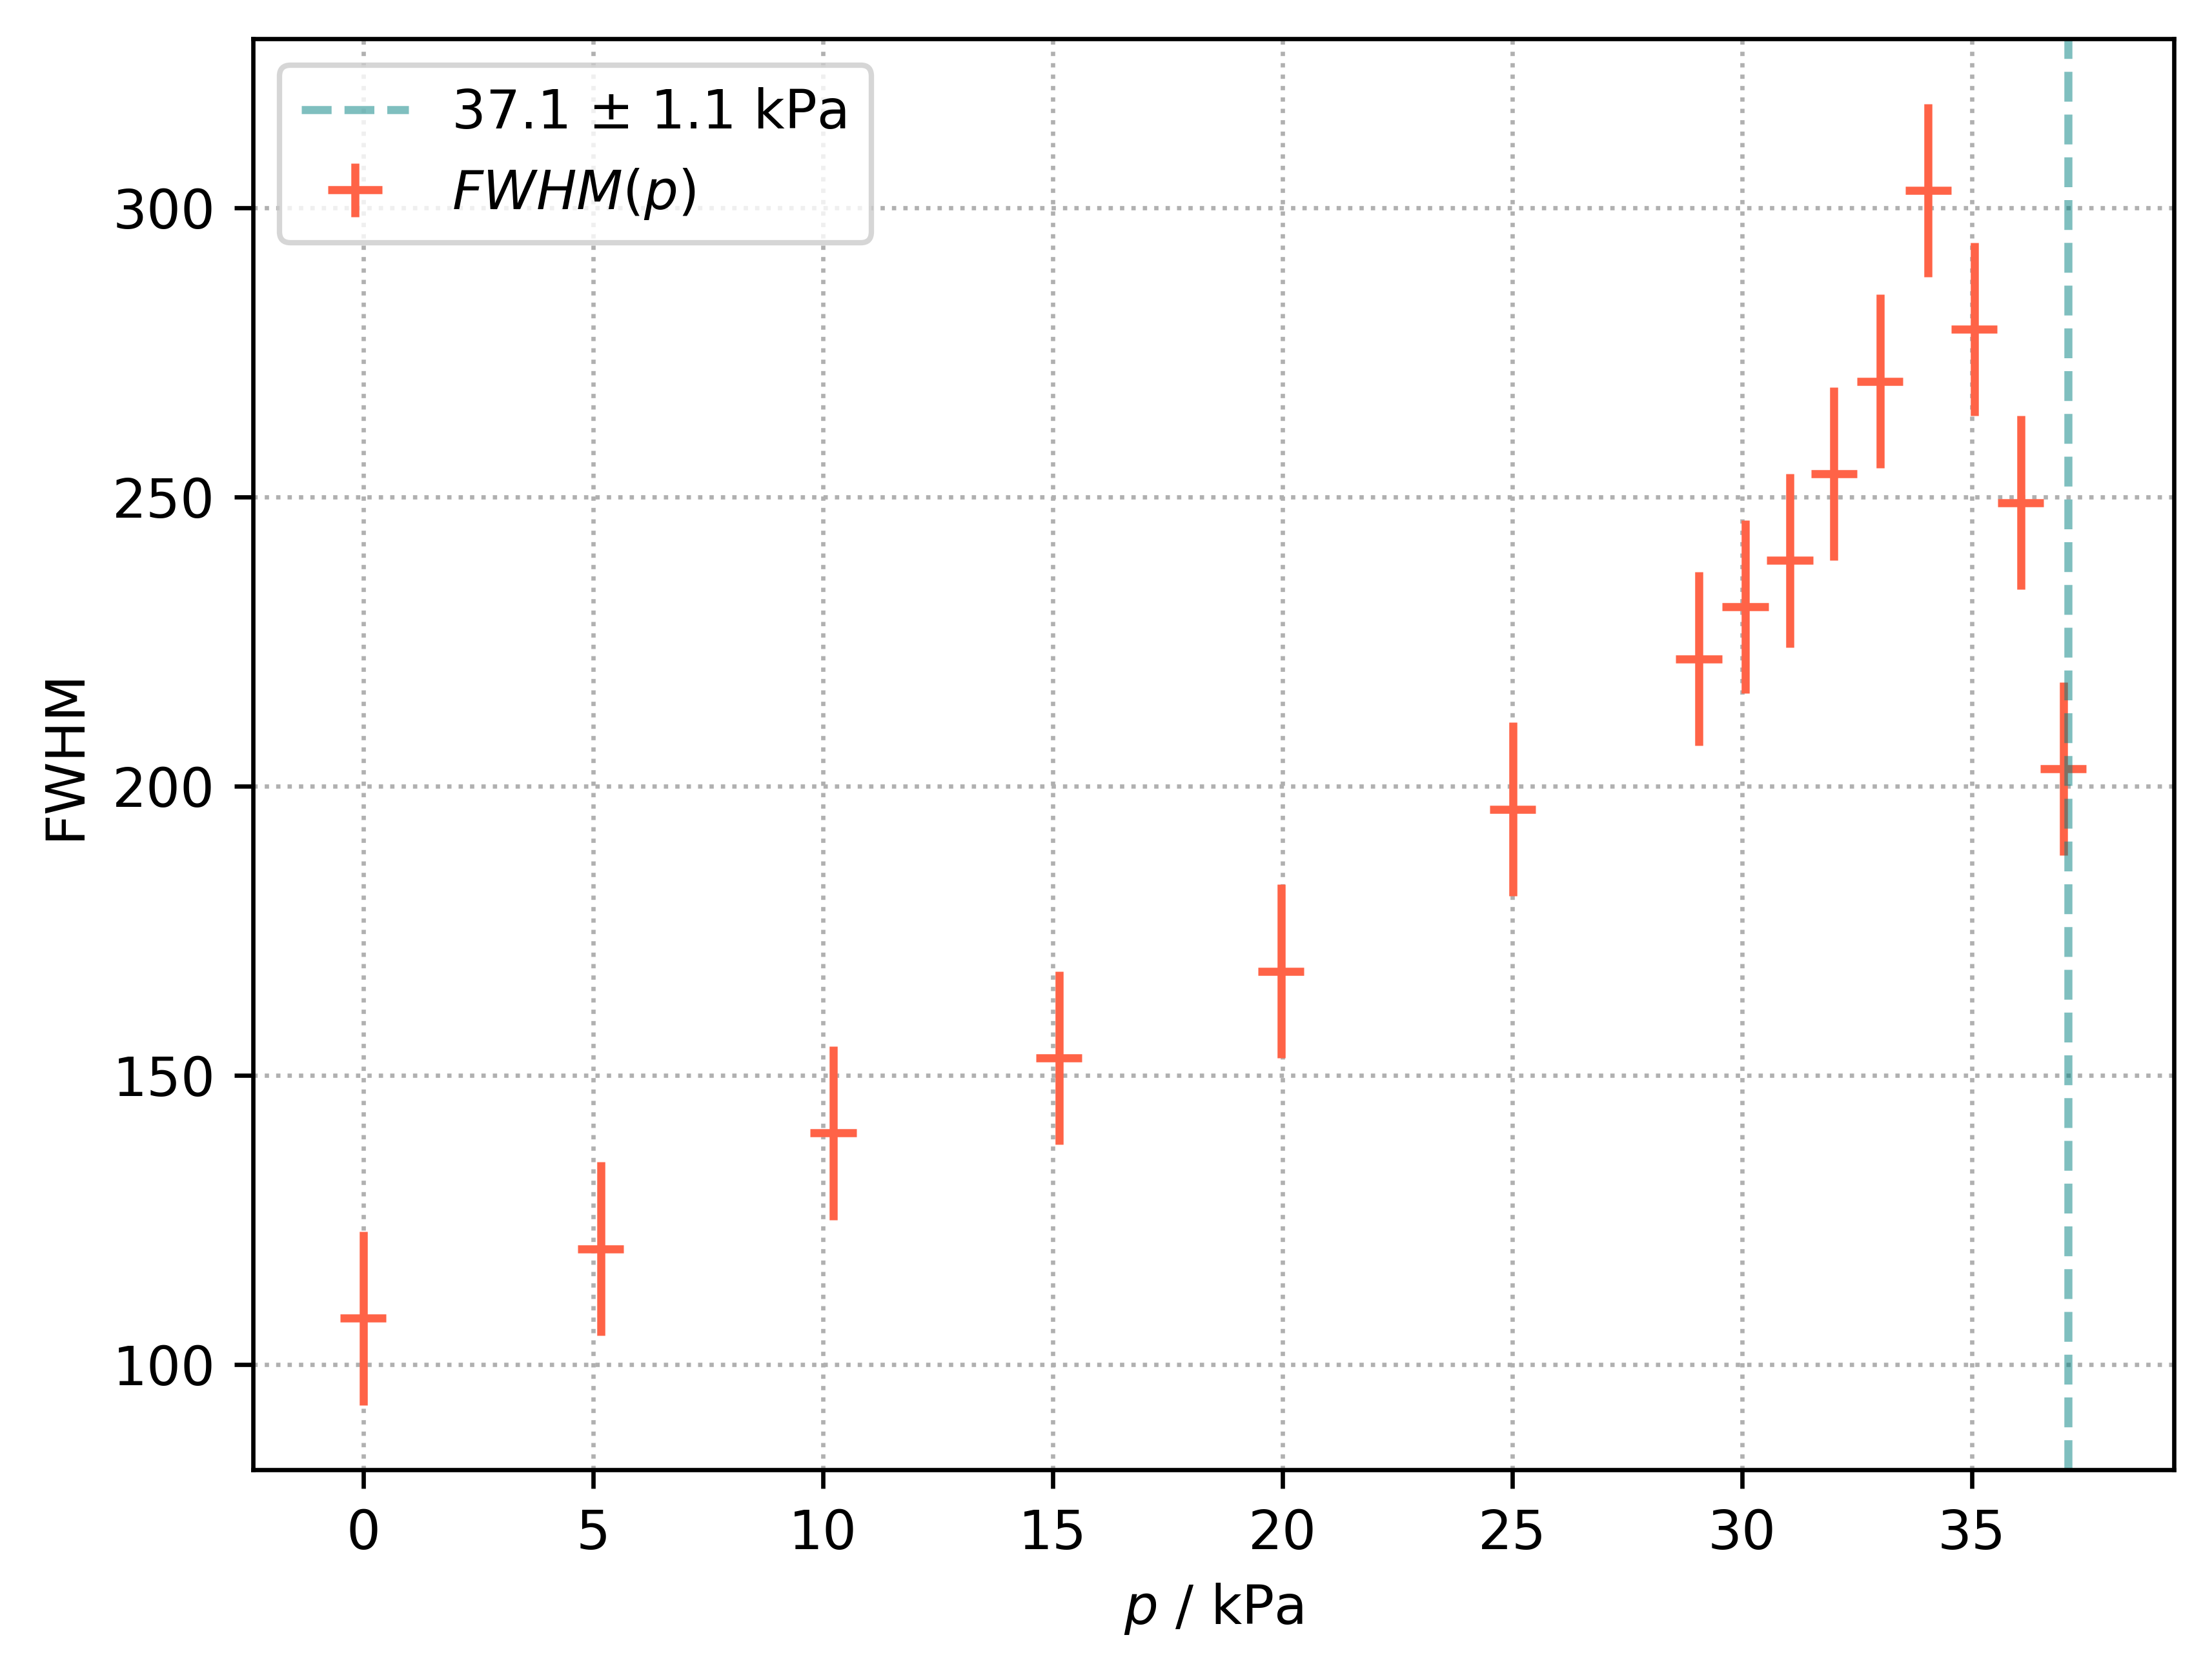
\includegraphics{FWHM_vs_pressure.png}
}}
\caption{Using our gaussian smoothing method we obtained the FWHM of the first fifteen spectra.
First, we find the maximum count in each smoothed spectrum and assign the corresponding index to a bin, we then calculate the half maximum count and from this, we find a position for the left bin (L) (corresponding to the left width of the peak). 
We find the index of the result of the counts up to the maximum count minus the half maximum all squared. Similarly for the right handed bin (R) but we offset the calculation by the bin corresponding to the maximum count value. Finally we substract the left bin (L) from the right bin (R) to find the FWHM of each spectrum. In the Figure we can see the uncertainty in the FWHM as a function of pressure is a visual estimate (ie. FWHM(p)$\pm 15$bins).
}
\end{SCfigure}

\begin{SCfigure}
\subfloat[]{\scalebox{0.5}{
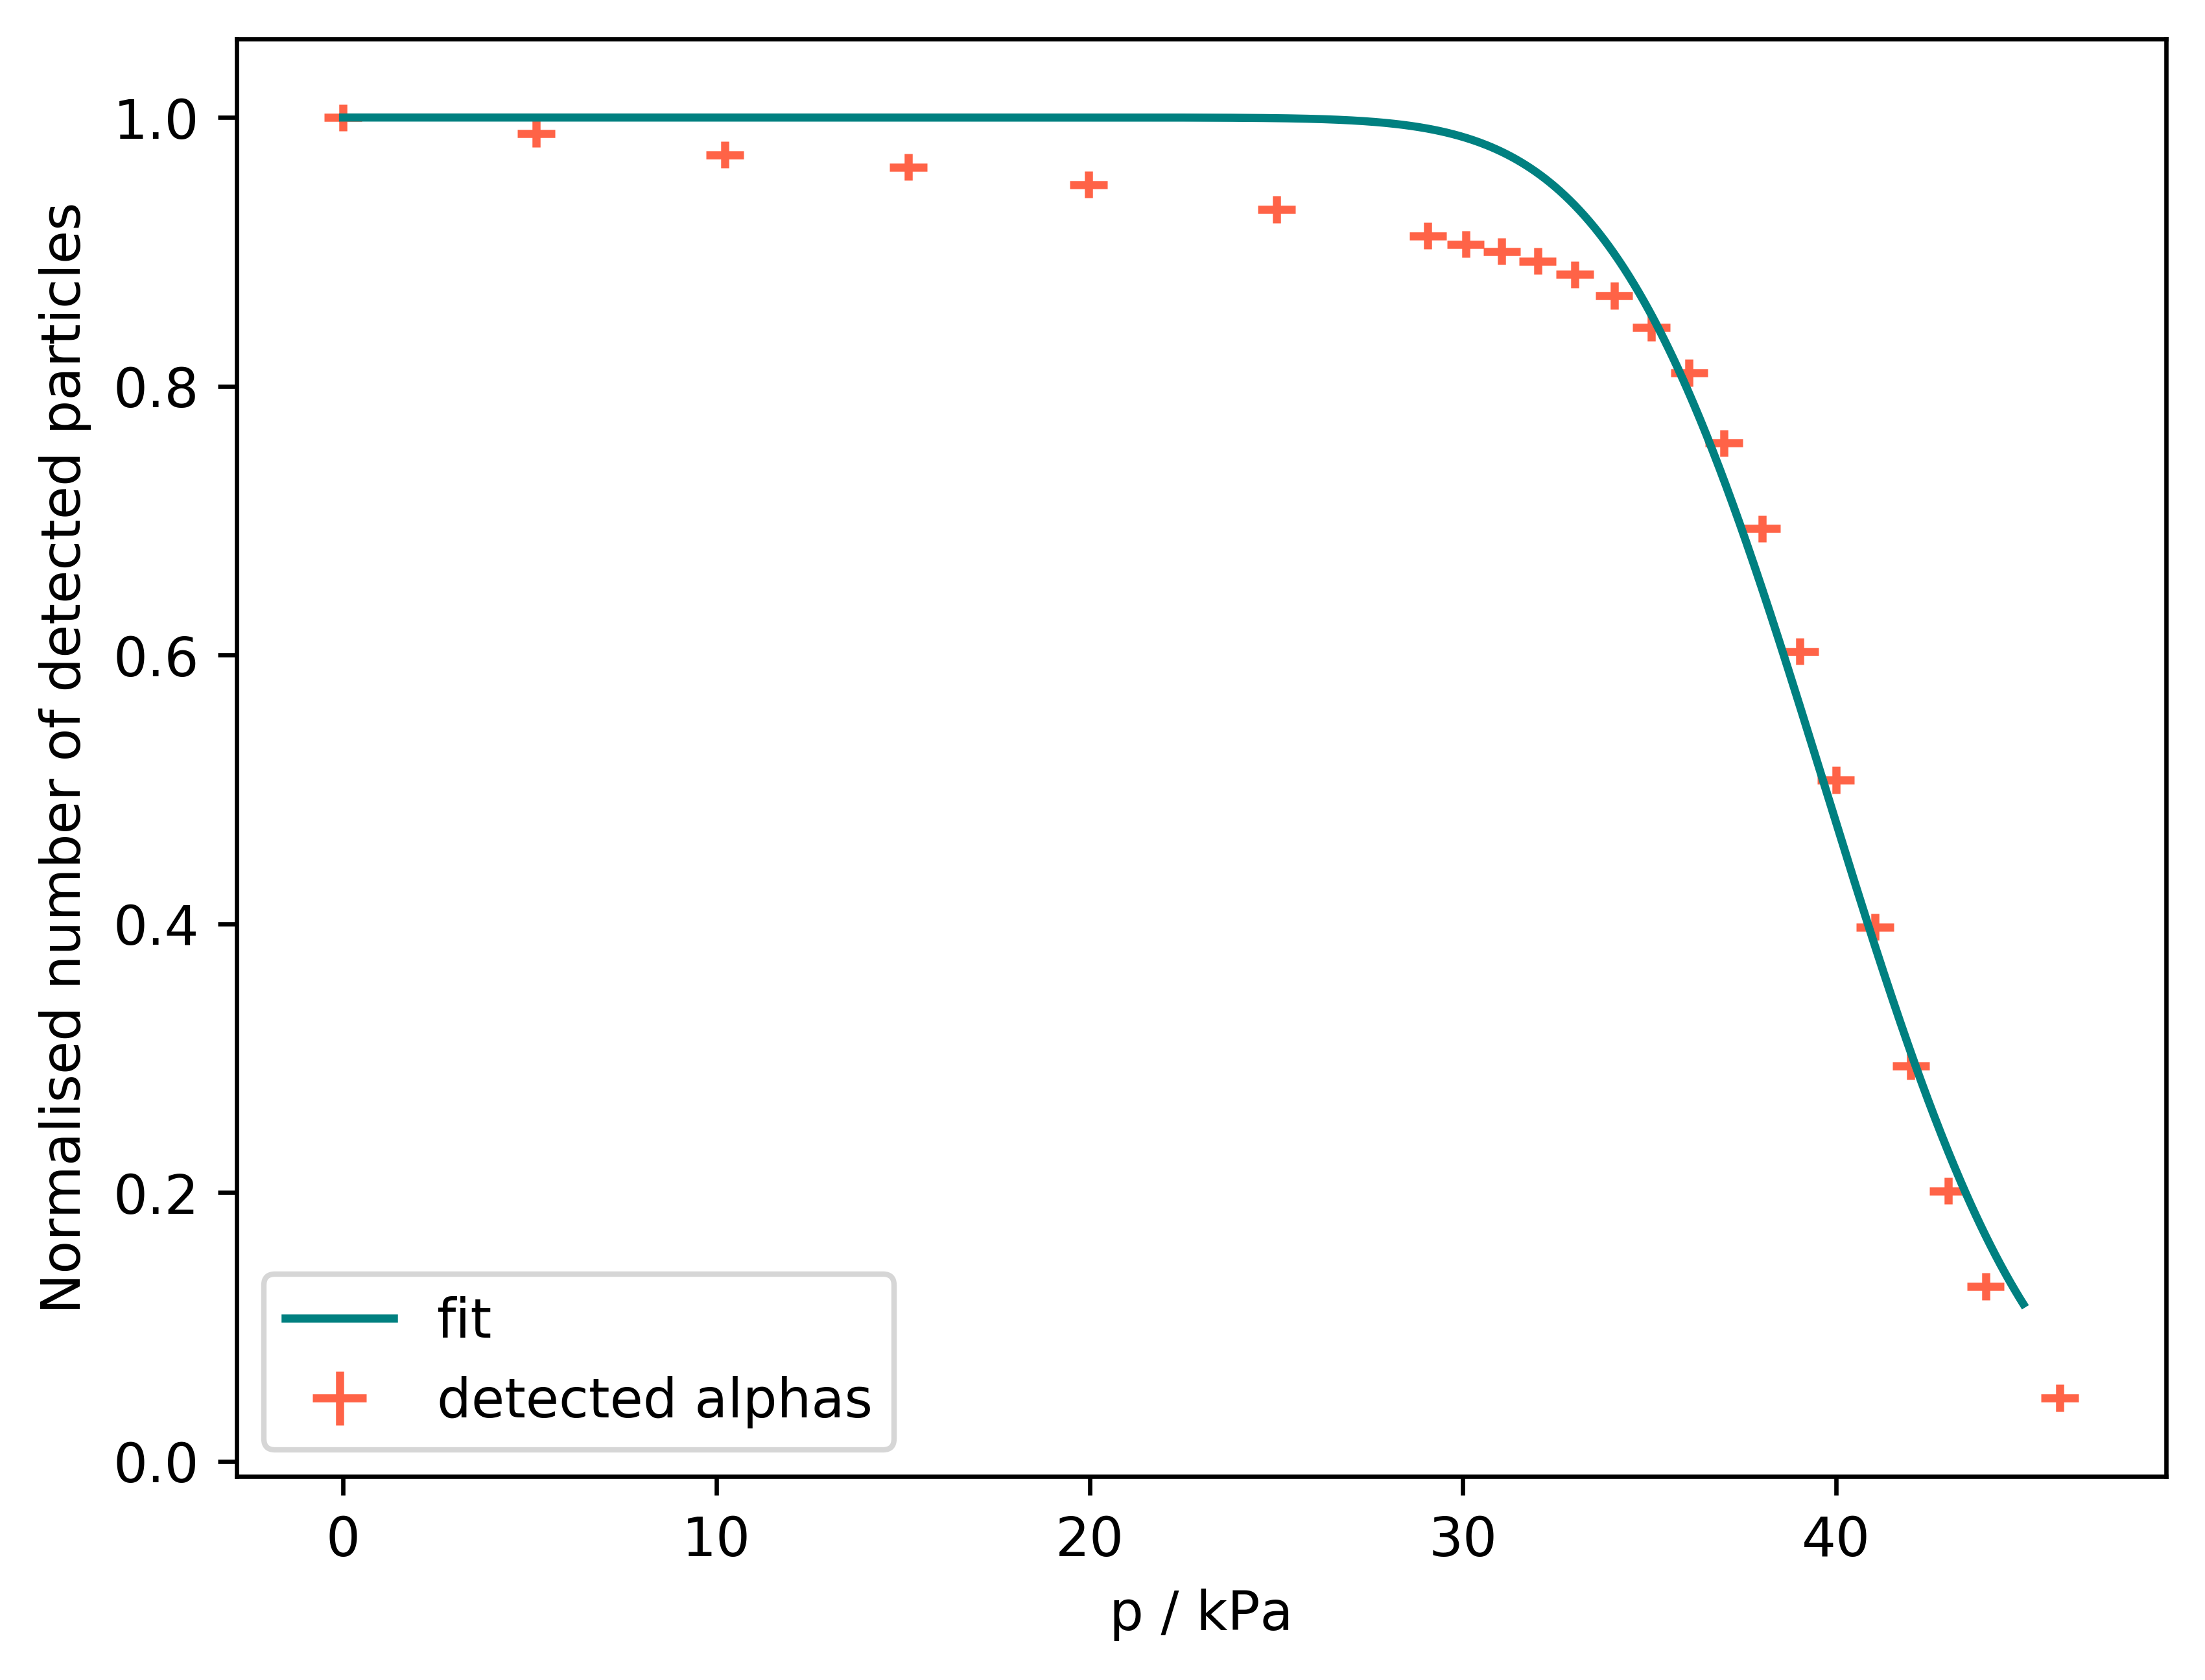
\includegraphics{alphas_vs_pressure.png}
}}
\caption{
We use the normalised number of detected particles (normalised to the first spectrum area) as a function of pressure.
From this fit the value of the straggling parameter is $\alpha = 0.15 \pm 0.01 cm$ 
The total radioactive counts are found by adding the counts in each spectrum (including the extrapolated region). Our fit is not very representative in the plateau region since it is expected that none of the alpha particles are lost at low pressures (Please see discussion). 
}
\end{SCfigure}


\clearpage
%-----------------------------------------------------------------------------------------
From our fit we also obtain the value for the zero energy pressure $P_0 = 39.72 \pm 0.18$ kPa whilst our previous result was $P_0: 37.1 \pm 1.1$kPa.
%-----------------------------------------------------------------------------------------

\begin{multicols}{2}
\section{Discussion}
The width of the energy peaks compared to the energy resolution of the detector requires us to consider the implications of changing the number of bins used. A smaller number of bins gives a higher count in each bin, which improves the signal to noise ratio in each bin since the uncertainty goes as the square root of the number of counts.
A larger number of bins gives a higher resolution of the spectrum, allowing us to find the centre more accurately, but the uncertainty in each bin height becomes bigger by the same reasoning as above\cite{feedback}.
Most of the spread in our spectra is likely due to the alpha particles travelling through the gold layer that is part of the radioactive source construction. 

The value of the straggling parameter $\alpha$ is expected to be $\alpha \cong k R_{atm} = 0.0370 \pm 0.0013$cm\cite{SPA}, whilst we find experimentally that $\alpha = 0.15 \pm 0.01$ cm this discrepancy must be a consequence of the construction of the radioactive source.
Since the particles must travel through at least $\Delta x = 2.45 \pm 0.08\mu$m. It is likely that the gold layering increases the straggling parameter by approximately a factor of 5. Clearly due to the fact that alpha particles are highly ionising, they are unable to penetrate very far through gold. 

The number of surviving particles varing with pressure demonstrates the effect of range straggling of alpha particles in air. It can be seen in Figure 7 that the total number of detected particles in each spectrum does not in fact satisfy our expectation at the low pressures region. In theory it is expected that nearly all alpha particles emmitted from the source would be detected at low chamber pressures but we don't see this behaviour. Instead we see that even at low pressures the number (normalised) of particles detected decreases.
Given the experimental setup, this behaviour remains unexplained. since the radioactve source is not a beam we cannot explain the decrease in detected particles due to a "warm up" process that a sort of beam instrument could experience as it is operational.


\section{Conclusion}
We measured the straggling parameter of alpha particles travelling in a pressure controlled chamber. The value of the experimental straggling parameter $\alpha = 0.15 \pm 0.01 cm$ is highly discrepant with the theoretical prediction $\alpha = 0.0370 \pm 0.0013$cm\cite{SPA}.
In addition to this result, we found that the value for the range pressure is $p_0 = 39.72 \pm 0.18$kPa.

\end{multicols}
\bibliography{mybib}
\bibliographystyle{unsrt}
\end{document}